% !TEX program = xelatex
\documentclass[12pt,oneside]{report}			% Začátek dokumentu

\usepackage{verbatim} %pro kód a multi-line komentáře
\usepackage{SP}							% Import stylu

\newcommand{\source}[1]{\caption*{Zdroj: {#1}} } %jedna z možnoszí citace obrázků

\newcommand{\doubleref}[1]{\ref{#1} na straně \pageref{#1}}

\usepackage{outlines} %pro nested listy

\lstset{
  basicstyle=\ttfamily,
  columns=fullflexible,
  frame=single,
  breaklines=true,
  postbreak=\mbox{\textcolor{gray}{$\hookrightarrow$}\space},
  backgroundcolor=\color{white},
  showspaces=false,
  showstringspaces=false,
showtabs=false,
}
\renewcommand\lstlistlistingname{Zdrojové kódy programů}

\usepackage{longtable} % for 'longtable' environment
\usepackage{pdflscape} % for 'landscape' environment

\author{Jakub Ambroz}
\title{Umělá inteligence a \gls{OCR}}
\date{19. února 2020}
\vedouci{Dr. rer. nat. Michal Kočer}
\place{V~Českých Budějovicích}
\skolnirok{2019/2020}
\logo{
\includegraphics[scale=0.75]{logo_gymji.jpg}}

\begin{document}

	\mytitlepage						% Vygenerování titulní strany
	
	\prohlaseni{
		Prohlašuji, že jsem tuto práci vypracoval samostatně s~vyznačením všech použitých pramenů.
	}	
	
	\abstrakt{ 
% Abstrakt
	Umělá inteligence je pojem zahrnující široké spektrum přístupů a algoritmů a některé z~nich jsou zde popsány. V~dnešní době má \gls{AI} spoustu využití. Jedno ze starších je rozpoznávání znaků v~textu, protože digitalizace tištěných dat umožní jejich strojové zpracování. Toto optické rozpoznávání znaků (\gls{OCR}) už má mnoho existujících řešení a jedno z~nich je Tesseract. V~praktické části je cílem zjistit, zda-li a jak je možné jeho výkon vylepšit úpravou vstupních obrázků pomocí OpenCV.
	}{ 
		\gls{OCR}, Optické rozpoznávání znaků,  \gls{AI}, Umělá inteligence,  OpenCV,  Tesseract, \gls{B-MOD}, Brno Mobile OCR Dataset,  předzpracování, preprocessing	% Klíčová slova
	}
	
	\podekovani{
	% Poděkování
	 Děkuji komunitě \LaTeX u za pomoc s~formální stránkou práce, zejména Jonáši Havelkovi a \href{https://tex.stackexchange.com/}{\emph{tex.stackexchange}}. Dále děkuji Pythonovské komunitě  \href{https://stackoverflow.com/}{\emph{stackoverflow}} za archiv zodpovězených otázek. \href{https://pero.fit.vutbr.cz/brno_mobile_ocr_dataset}{\emph{\gls{B-MOD}}} za správně označený dataset. A v~neposlední řadě tvůrcům nástrojů  \href{https://tesseract-ocr.github.io/tessdoc/Documentation}{\emph{Tesseract}} a \href{https://opencv.org/}{\emph{OpenCV}} a autorům přidružených dokumentací a návodů. \\
	A~především děkuji svému vedoucímu práce za trpělivost při kontrole maturitních prací, za pomoc s~výběrem tématu a všeobecně dobrý a podporující přístup.
	}
	
	\tableofcontents\newpage			% Obsah
	
	
	
	
	\chapter{Úvod}
		Umělá inteligence se vždycky vyznačovala tím, že vnímání toho, co je a není \gls{AI} se měnilo podle toho, čeho byla aktuálně schopná. Jakmile bylo dosáhnuto nějakého obtížného cíle, tak se usoudilo, že k~jeho dosažení není potřeba inteligence, že je to jen statistika nebo předprogramovaný algoritmus, takže se už nejedná o~doménu \gls{AI}.\\
		V~této práci jsou nastíněny techniky rozpoznávání znaků. Některé z~nich už bychom dnes mezi \gls{AI} neřadily. Naopak \gls{napr} neuronové sítě se dnes těší velkému zájmu, ale asi ne z~důvodu využití v~\gls{OCR}.\\
		V~praktické části využiji již předtrénovanou \gls{NS} k~rozpoznávání znaků. Bude to Tesseract 4.0, přesněji pytesseract, který nám umožní využívat Tesseract z~pohodlí Pytohnu. Pokusím se vytvořit program, který zjistí, jak zlepšit úspěšnost rozeznávání znaků, pomocí úpravy obrázků. Na práci s~obrázky použiji knihovnu OpenCV.\\

		
	
	\part{Teoretická část}
	\chapter{OCR}
	\label{sec:OCR}	
	OCR je zkratka \gls{en} \emph{Optical Character Recognition} (v~češtině optické rozpoznávání znaků \parencite{wiki:OCR}) je proces rozpoznávání a klasifikace vzorů v~digitálním obrázku.\parencite[\gls{s} 9]{chaudhuri2017optical}\\
	Oblasti rozpoznávání znaků:
	\begin{outline}
	 	\1 On-line - rozpoznává znaky, hned jak jsou nakresleny
     	\1 Off-line - rozpoznává až potom, co je tisk (nebo psaní) dokončený
     		\2 Samostatné znaky
     			\3 Tištěné
     			\3	Ručně psané
     		\2 Ručně psané psací písmo
     			\3 Rozpoznání
     			 \3 Ověření
	\end{outline}
	\parencite[\gls{str} 12]{chaudhuri2017optical}, \parencite[\gls{str} 7]{eikvil-ocr}

	\subsubsection{Historie}
	\label{sec:OCR-history}
	 Vývoj \gls{OCR} systému již v~50. letech 20. století a zpočátku zvládali jen specializované symboly pro čtení počítačem. Později byly stroje pouze omezené v~počtu fontů, protože používali metodu shody šablon (\gls{en}  \emph{template matching}), která porovnávala obrázek znaku s~knihovnou s~šablonami každého znaku z~každého fontu. Bylo vyvinuto velké úsilí na standardizaci fontů, \gls{viz} obrázek \ref{fig:ocr-font}. Vývoj se nakonec ubral k~systémům schopným rozeznat více fontů. S~klesající cenou a rostoucím výkonem hardwaru se stali komerčně dostupné a v~90. letech se techniky \gls{OCR} spojili s~výzkumem v~oblasti \gls{AI}. Dnešní systémy dosahují velmi uspokojivých výsledků. Jako jedno z~posledních míst s~možností výrazného zlepšení zbývá ručně psaný text. \parencite[\gls{s} 8-10]{eikvil-ocr}, \parencite[\gls{s} 15]{chaudhuri2017optical}
	\begin{figure}[h]
	\centering
	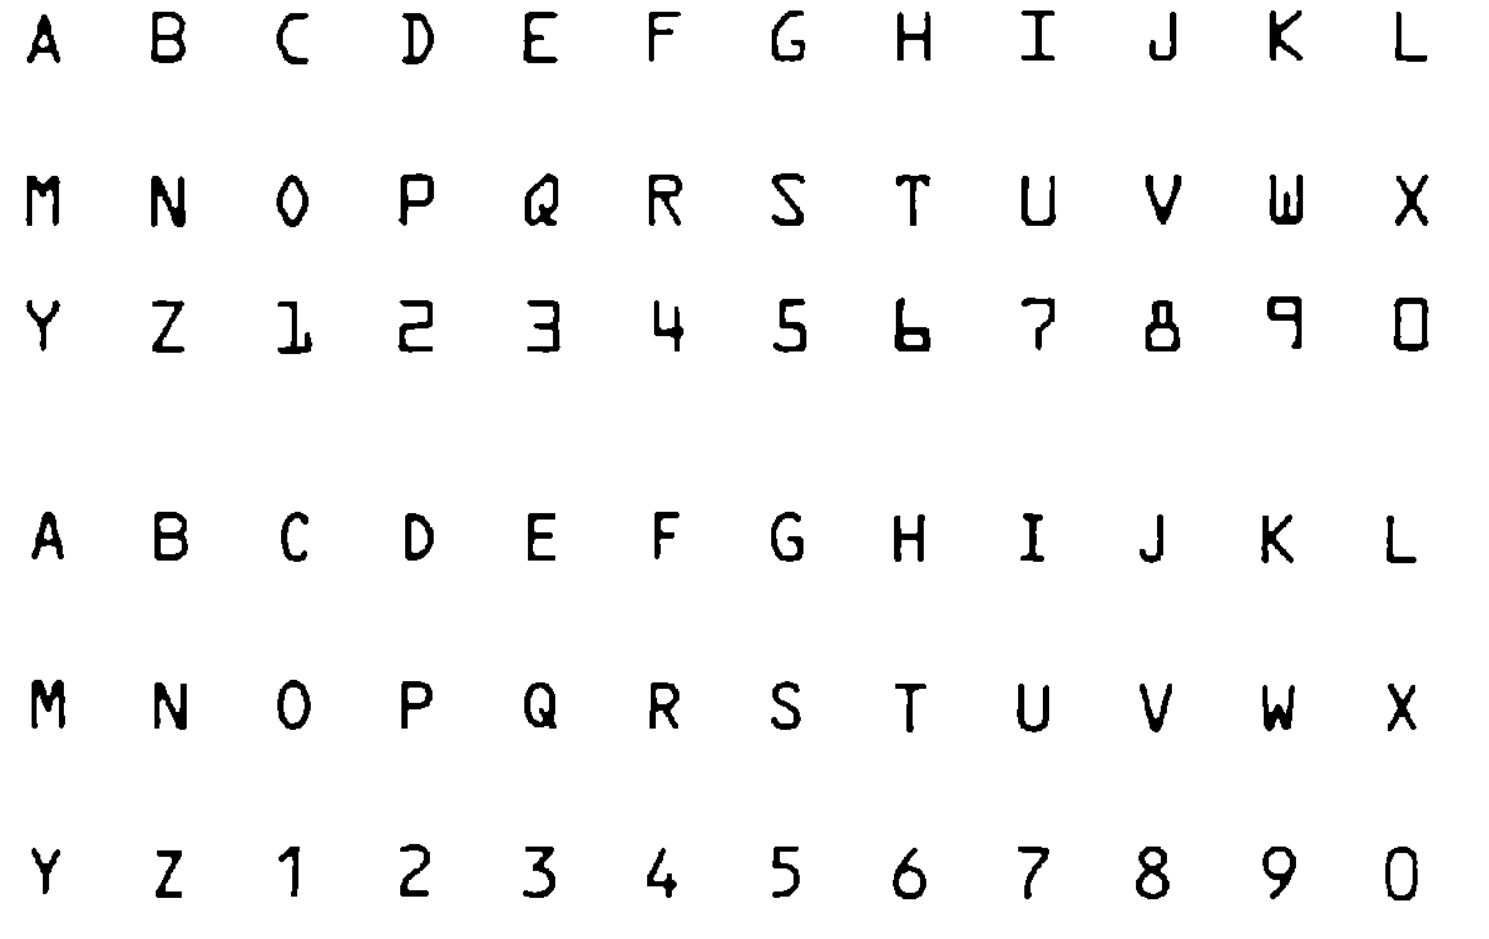
\includegraphics[scale=0.15]{OCR/font-a-b}
	\caption{Standardizované fonty americký OCR-A (nahoře) a evropský OCR-B (dole), zdroj: \parencite[\gls{str} 9]{eikvil-ocr}}
	\label{fig:ocr-font}
	\end{figure}
		
	\section{Techniky \gls{OCR}}
	\label{sec:OCR-techniky}	
	\subsection{Skenování}
	\label{sec:scan}
	Proces \emph{optického skenování} zachycuje digitální obraz původního dokumentu. Zařízení nazývané OCR skener obsahuje senzorické čidlo, které převede intenzitu světla do úrovní šedi (\gls{en} \emph{grayscale}). Protože jsou obvykle tištěné dokumenty černobílé, převádí se více-úrovňový obrázek do binárního, který má místo jen více úrovní šedi jen 2 hodnoty (proto se nazývá binární nebo dvou-úrovňový) a to černou a bílou. Tento proces, který se nazývá \emph{thresholding} (z~\gls{en} slovíčka pro práh, threshold), protože jednotlivé pixely označí za černé (resp. bílé) překročí-li úroveň šedi určitý práh, se často vykonává již v~samotném skeneru, protože to šetří místo v~paměti a výpočetní náročnost. \parencite[\gls{str} 12]{eikvil-ocr} \\
	Thresholding je důležitý proces, protože na kvalitě binárního obrázku jsou závislé rozpoznávací schopnosti systému. Jednotný práh v~rámci celého obrázku může být dostatečný, pokud má dokument dostatečně kontrastní a jednotné pozadí, ale mnoho dokumentů v~praxi tyto podmínky nesplňuje. V~těchto případech je třeba sofistikovanějších metod pro kvalitní výsledky. Ty nejlepší techniky přizpůsobují práh podle lokálních vlastností (jako kontrast a jas) dokumentu, ale proto také často vyžadují víceúrovňové skenování dokumentu. \parencite[\gls{str} 16-17]{chaudhuri2017optical}
	\subsection{Lokace a segmentace}
	\label{sec:locate-segment}
	Proces segmentace určuje složky obrázku. Zajišťuje rozlišení a lokalizaci textu a ostatních částí (\gls{napr}: grafy, loga, obrázky). Segmentace izoluje samostatná slova nebo znaky. Většinou se slova rozdělují na izolované znaky, které jsou rozpoznávány jednotlivě. Obvykle se izolují spojené součásti, protože je to jednoduché na implementaci. Ale může dojít k~problémům, pokud se znaky dotýkají nebo jsou naopak rozdělené na více částí. \parencite[\gls{str} 17]{chaudhuri2017optical}
	Nejdůležitější úkoly mohou být rozděleny do 4 kategorií \parencite[\gls{s} 13]{eikvil-ocr}:
	\begin{enumerate}
	\item{Rozpoznání dotýkajících se a rozdělených znaků:\\ Několik znaků může být omylem spojeno v~jeden z~pohledu \gls{OCR}, pokud je skenování provedeno na příliš nízkém prahu. Některé fonty (patkové) jsou k~tomuto náchylnější. Při roztříštění znaku dojde k~mylnému určování každé části jako samostatného znaku.}
	\item{Oddělení šumu od textu:\\ Zejména problém pro tečky a čárky.}
	\item{Záměna grafických prvků a textu:\\ Pokud je grafika zaměněna za text, dojde k~odeslání netextu k~rozpoznání, což přidá nesmyslné části do výstupu. Pokud je text zaměněn za grafiku, bude část výstupu chybět.}
	\end{enumerate}
	
	\subsection{Předzpracování}
	\label{sec:Preproces}
	Cílem \emph{předzpracování} (\gls{en} preprocessing) je provést takové změny, aby byla úspěšnost rozeznání vyšší. Obrázek získaný procesem skenování může obsahovat šum a jiné defekty, které kazí rozpoznávání. Nejběžnější je technika nazývaná \emph{vyhlazování} (\gls{en} \emph{smoothing}), která zahrnuje \emph{vyplňování} (\gls{en} \emph{filling}), které odstraňuje malé díry a mezery ve znacích, a \emph{zeštíhlení} (\gls{en} \emph{thinning}), které zmenší tloušťku čáry. Na vyhlazování se obvykle používá okno, které se posouvá po binárním obrázku a na jeho obsah jsou uplatněna určitá pravidla. Další technikou je \emph{normalizace}, která má za cíl sjednotit znaky ve velikosti, sklonu a rotaci. Do předzpracování se zahrnuje i komprese, která ale zachovává všechny potřebné informace pro OCR. \parencite[\gls{s} 17-18]{chaudhuri2017optical}			
	
	\subsection{Segmentace}
	\label{sec:extraction}
	Předzpracování nám dá čistý obrázek, který je bez šumu a obsahuje dostačující množství informací. Segmentace odděluje různé čáry a přímo tak ovlivňuje úspěšnost rozpoznávání. \emph{Vnitřní segmentace} (\gls{en} internal segmentation) se zaměřuje na spojované písmo a jeho rozdělení do čar a křivek. Zatím se jedná o~nevyřešený problém, přestože bylo objeveno mnoho dobrých metod. Existují přístupy explicitní, implicitní a smíšené, které jsou nejúspěšnější.\parencite[\gls{s} 22]{chaudhuri2017optical}
	\subsection{Reprezentace}
	Reprezentace je proces, který získá \emph{rysy} z~každé kategorie, které pomohou rozlišit tuto kategorii od jiných, ale zároveň tyto nejsou ovlivněny obvyklými rozdíly v~rámci této kategorie. Cílem je získat, co nejvíce reprezentativní informace z~prvotních dat.
	\begin{itemize}
	\item{\emph{Globální transformace} a \emph{rozšíření série} (\gls{en} \emph{series expansion}):\\Signál obvykle obsahuje více informací, než je potřeba. Jedním ze způsobů je reprezentovat signál lineární kombinací sérií jednodušších a dobře definovaných funkcí.}
	\item{\emph{Statistická reprezentace}:\\ Reprezentuje znak statistickým rozdělením bodů. Není možné zrekonstruovat původní obraz, protože zmenšuje rozměry sady znaků a tím zvyšuje rychlost a snižuje složitost.}
	\item{\emph{Geometrická a topologická reprezentace}: \\Různé vlastnosti znaku mohou být reprezentovány geometrickým nebo topologickým způsobem, které mají velkou odolnost proti zkreslení. Tento způsob popisu také umožňuje získat znalosti o~struktuře objektu nebo jeho dílčích částí.}
	\end{itemize}
	\parencite[\gls{s} 23-28]{chaudhuri2017optical}
	\subsection{Získávání rysů znaku}
	Získávání rysů (\gls{en} \emph{feature extraction}) je považována za jeden z~nejnáročnějších problémů rozpoznávání vzorů. Cílem je získaní hlavních a nezbytných vlastností znaku. Ty se vybírají na základě jejich odolnosti proti šumu, zkreslení, rotaci a praktickému využití, \gls{tj} rychlost rozpoznání, náročnost implementace. Na získávání rysů je přímo navázaná jejich \emph{kategorizace} (neboli klasifikace), která identifikuje znak. \parencite[\gls{str} 28-29]{chaudhuri2017optical}
	\subsection{Rozpoznávání a trénování}	
	Využitím metod \emph{rozpoznávání vzoru} (\gls{en} \emph{pattern recognition}), které přiřadí neznámý vzorek do předdefinované kategorie. Základní rozdělení je na čtyři přístupy, které nejsou nezávislé a může se stát, že technika z~jednoho přístupy může být také považována za techniku jiného přístupu. První je \emph{porovnání se šablonou} (\gls{en} emph{template matching}), které porovnává znak se sadou vzorových znaků (\gls{tj} šablon). Může taky využívat deformovatelných šablon. \parencite[\gls{s} 29-34]{chaudhuri2017optical}\\
	Druhým je \emph{technika statistická}, která využívá rozhodovací funkce a sadu optimálních kritérií, které maximalizují pravděpodobnost výskyt pozorovaného vzoru v~určité kategorii. Využívá se více statistických přístupů \gls{napr}: skrytý Markovův model, mlhavou logiku (\gls{en} fuzzy reasoning \gls{viz} \ref{sec:fuzzy}) nebo shlukové analýzy (\gls{en} cluster analysis). \parencite[\gls{s} 29-34]{chaudhuri2017optical}\\
	\emph{Strukturální techniky} rekurzivně popisuje složitější vzory jednoduššími. Pomocí těchto vzorů jsou popsány a kategorizovány znaky. Dělí se na metody, které využívají gramatické, které využívají lingvistická pravidla, a grafické.
	V~neposlední řadě se využívají \emph{\gls{ANN}}, které jsou schopné adaptovat se změnám v~datech. Přestože využívají jiných vnitřních přístupů jsou \gls{ANN} porovnatelné se statistickými technikami. \parencite[\gls{s} 29-34]{chaudhuri2017optical}
	\subsection{Následné zpracování}
	\label{sec:postproces}
	\Gls{en} \emph{postprocessing} (nebo post-processing) by se dalo přeložit jako následné zpracování nebo \emph{pozpracování}. První částí je \emph{seskupování} (\gls{en} \emph{grouping}) jednotlivých znaků v~textové řetězce na základě jejich pozice v~dokumentu. Je nutné rozlišit, jestli je mezera mezi znaky jen mezerou mezi znaky nebo mezerou mezi slovy, aby bylo možné seskupit znaky do slov. Protože jsou mezery mezi slovy výrazně větší, tak to není příliš obtížné ani pro méně vhodné fonty. Skutečné problémy nastávají, pokud se jedná o~ručně psaný text (nepravidelná velikost mezer) a nebo pokud je text zkreslený.\parencite[\gls{s} 20]{eikvil-ocr}\\
	Po seskupení znaků ve slova můžeme v~druhé části následného zpracování využít kontextu, kde se znak nachází, k~nalezení a opravení některých chyb. Žádný, ani ten nejlepší, \gls{OCR} systém nemá schopnost rozpoznat 100\% znaků správně. První způsob využívá \emph{pravděpodobnost výskytu sledu znaků společně}. \Gls{napr} za tečkou předpokládáme velké písmeno. Navíc může být vypočítána pravděpodobnost výskytu 2 znaků za sebou, to se samozřejmě liší podle jazyka (\gls{napr} v~češtině můžeme předpokládat, že znak "ě" po písmenu "j" nebo libovolné měkké souhlásce, je pravděpodobně chyba).Dalším přístupem je využití \emph{slovníků}, ve kterých se vyhledá slovo. Pokud takové slovo neexistuje, je nalezena chyba, která může být opravena upravením slova na nejvíce podobné. To, že je slovo je nalezeno existenci chyby nevylučuje, protože mohlo dojít k~záměně na jiné existující slovo. Přesto je tato metoda nejefektivnější pro nalézání a opravu chyb, přestože je časově náročná. \parencite[\gls{str} 20-21]{eikvil-ocr}
	
	\section{Soft computing}
	\label{sec:soft}
	Soft computing (z~\gls{en} do češtiny by se dalo přeložit jemné výpočty) se ukázalo jako možné cenově efektivní řešení v~podobě \gls{OCR} systémů. Do soft computing spadají lidským mozkem inspirované metodologie, které mají za cíl využít toleranci k~nepřesnostem a k~nejasnostem k~dosažení robustnosti a nízkých nákladů. Základními zástupci jsou mlhavá logika (\gls{viz} fuzzy logika \ref{sec:fuzzy}), neuronové sítě (\gls{viz} \gls{NS} \ref{sec:NN-uvod}), pravděpodobnostní logika a genetické algoritmy (\gls{viz} \ref{sec:genetic}). Jednotlivé typy nejsou konkurenti, ale spíš se vzájemně doplňují a jejich kombinování je výhodné. Využívá se pro \emph{NP-úplné problémy}, \gls{tj} problémy, u~kterých se předpokládá, že neexistuje žádné polynomiální algoritmus k~jejich řešení.  \parencite[\gls{str} 43-45]{eikvil-ocr}, \parencite[\gls{str} 48-49]{soft_fuzzy}
	
	\section{OCR dnes}
	\label{sec:ocr_today}
	V~dnešní době je velké množství \gls{OCR} systémů. Většina z~nich je cílená jen na zdigitalizování tištěných dokumentů, takže pokud chceme \gls{OCR} s~širším využitím, máme možnost využít služeb (placených) od technických gigantů, jako je \emph{Microsoft} (počítačové vidění pod Azure, kde nabízí cloudové výpočty), \emph{Google} (Vison AI pod Google Cloud) a \emph{Amazon} (služba Rekognition). Ti kromě vlastních speciálních algoritmů využívají svých obrovských výpočetních kapacit a zapůjčují je k~analýze obrázků. Kromě textu jsou tyto systémy schopny rozeznávat objekty, obličeje nebo i nevhodnost obrázku. \parencite{MS_CV}, \parencite{Google_CV}, \parencite{Amazon_CV}
	
	
	
	\chapter{Umělá inteligence}
	\label{sec:AI}
	Umělá inteligence (\gls{en} artificial intelligence, \gls{zkr} \gls{AI}) je obor, který se snaží uměle vybudovat inteligentní systémy. Existuje mnoho možných přístupů. Některé se zaměřují na myšlení a uvažování těchto systémů , jiné na jejich chování a akce. \gls{AI} může být buď porovnáváno s~lidským výkonem nebo oproti ideálnímu výkonu, nazývanému racionalita.\\
	\emph{Turingův test} spočívá v~testování, zdali je člověk schopen \gls{AI} rozlišit od člověka na základě textové komunikace. To vyžaduje, aby byl počítač schopen pracovat s~jazykem, pamatovat si viděné a slyšené, schopnost uvažování (\gls{napr} odpovídat na otázky) a učení. Tento přístup se řadí do kategorie \emph{lidské konání} (\gls{en} \emph{Acting humanly}). Naproti tomu přístup \emph{lidského myšlení }(\gls{en} \emph{Thinking humanly}) se snaží replikovat postupy a mechanismy lidského uvažování. To ale naráží na problém, že musíme dobře porozumět samotnému lidskému myšlení.\\
	\emph{Racionální myšlení} (\gls{en} \emph{Thinking rationally}) se snaží vytvořit dokonalý zdůvodňovací systém využívající logiku. Problém představuje zapsání některých dat správnou formální notací, obzvláště když jsou výroky méně než 100\% jisté, což je v~reálném světě (mimo matematiku) obvyklé. Dalším problémem je náročnost výpočtu.\\
	 Přístup \emph{racionálního konání} (\gls{en} \emph{Acting rationally}) definuje \emph{rozumné činitele} (neboli racionální agenty, \gls{en} \emph{rational agent}), které jednají tak, aby dosáhli nejlepšího možného výsledku, alespoň na základě dostupných informací. Tento přístup v~sobě může zahrnovat racionální myšlení, protože k~racionálnímu chování je v~některých případech třeba problém logicky vyřešit. Na rozdíl od lidského chování je to racionální obecnější a snáze matematicky definovatelné. Proto můžeme specifikovat jako cíl, kterého má racionální agent dosáhnout, lidské chování. V~mnoha případech ale není časově možné provést všechny výpočty. Toto je problém omezené racionality (\gls{en} \emph{limited rationality}).
	\parencite[\gls{s} 1-5,29-30]{AIAMA}


	\section{Hledání}
	\label{sec:search}	
	Mnoho problémů je řešitelné pomocí vhodného způsobu hledání. Ke správnému provedení potřebujeme dobře nadefinovat počáteční stav, všechny možné proveditelné akce, model přechodu, který řeší výsledky provedených akcí, cílový stav a funkci, která otestujte zda-li ho bylo dosáhnuto. Prostředí je reprezentováno \emph{polem stavů} (\gls{en} \emph{state space}). Cesta vedoucí z~počátečního stavu do cílového je řešení. Jeho efektivitu počítá účelová funkce (více o~ní \ref{sec:BP} u~backpropagace). Vyhledávací algoritmy považují stavy a akce za atomické, \gls{tj} dále nedělitelné, takže dále neřeší jejich vnitřní strukturu a nepracují s~ní.\parencite[\gls{str}]{AIAMA}
	
	\section{Učení}
	\label{sec:learning}	
	Učení je definováno \gls{napr} jako proces získání znalosti, pochopení nebo schopnosti zkoumáním, ukázkou nebo zkušeností. Nebo jako modifikace chování na základě zkušeností či nových znalostí. Využívá se, protože v~některých případech je nemožné nebo velmi složité vytvořit přesný algoritmus. \Gls{napr}  prostředí, ve kterém bude stroj operovat, není přesně popsané (nebo popsatelné) nebo se může v~čase měnit, tak místo ručního přizpůsobování algoritmu je lepší takový, který se je sám schopný adaptovat na měnící se podmínky. Další využití je v~\emph{dolování dat} (\gls{en} \emph{data mining}), kdy se snažíme najít vztahy a korelace v~obrovských množstvích dat. \parencite[\gls{s} 1-3]{introductionML}
	\subsubsection{Online a Offline}
	\label{sec:on-off-lol}
	Online přizpůsobuje síť (nebo algoritmus) po každém příkladu. Offline učení bere sadu problémů naráz a změnu provádí pro všechny najednou. Offline učení bývá také nazývané \gls{en} jako \emph{batch training procedures} (v~češtině zhruba dávkový nebo várkový trénovací postup), protože řeší celou dávku najednou. \parencite[\gls{s} 54]{NN_introduction-Kriessel} \\
	 % Alterntivně  \parencite[\gls{str} 720]{AIAMA}
	 
	\subsection{Rozdělení podle zpětné vazby}
	\label{sec:AI-deleni}
	\Gls{en} \emph{unsupervised learning} (v~češtině \emph{učení bez dohledu)} je metoda, při které dostane agent (\gls{napr} \gls{NS}) pouze vstupní data a sám bez jakékoliv zpětné vazby se snaží najít vzory v~datech a roztřídit je do kategorií. \parencite[\gls{s} 694-695]{AIAMA}, \parencite[\gls{str} 52]{NN_introduction-Kriessel}\\
	V~\gls{en} \emph{reinforcement learning} (česky \emph{zpětnovazební učení}) dostane agent informaci zda byl výsledek správný nebo špatný neboli dostane odměnu či trest. Tato metoda posiluje (nebo upevňuje, \gls{en} reinforcement) správné výstupy  a odrazuje od nesprávných. Proto je to efektivnější než učení bez dohledu. Agent sám ale musí přijít na to, jak změnit výstup \parencite[\gls{s} 695]{AIAMA}, \parencite[\gls{str} 53]{NN_introduction-Kriessel}\\
	V~\emph{učení s~učitelem} (\gls{en} \emph{supervised learning}) dostane kromě vstupních dat, také jejich správné řešení. Nevýhodou je, že vyžaduje, aby velké množství dat bylo předem správně označeno. Proto se v~praxi využívá kombinace těchto přístupů, protože máme jen málo příkladů správně označených a velké množství neoznačených či dokonce špatně označených. \parencite[\gls{s} 695]{AIAMA}, \parencite[\gls{str} 53]{NN_introduction-Kriessel}\\
	
	\section{Umělé neuronové sítě}
	\label{sec:NN-uvod}
	(Umělé) Neuronové sítě (\gls{zkr} \gls{NS}, \gls{en} (Artificial) Neural networks, \gls{zkr} \gls{NN} (/\gls{ANN})) jsou typem umělé inteligence. Jako vzor při jejich vytváření sloužily neurony (a jejich spojení) u~živočichů. Cílem je získání žádoucích vlastností biologických předloh, zejména: schopnost učení, tolerance kazů (\gls{tj} nepřesností nebo šumu ve vstupních datech) a schopnost zobecňovat a sdružovat data. \parencite[\gls{s} 3-5]{NN_introduction-Kriessel}\\
	Spojení neuronů je jednosměrné. Dendrity přijímají vzruchy z~různých neuronů. Při aktivaci neuronu se vyšle vzruch pomocí axonu do dalších neuronů. K~aktivaci neuronu dojde v~případě, že přijaté vzruchy překonají určitý aktivační \emph{práh} (\gls{en} \emph{threshold}).\parencite[\gls{str} 21]{NN_introduction-Kriessel}\\
	Tím získáme nejjednodušší model neuronu \eqref{eq:neuron0}, kde $n$ je počet vstupních spojení do neuronu a kde $a_i$ označuje výstup neuronu $i$. Neuron sečte všechny vstupní hodnoty a porovná, zda-li jsou větší než \emph{práh}. Pokud jsou, tak vyšle neuron výstupní signál s~hodnotou 1. A pokud je práh větší, nedojde k~aktivaci neuronu a ten tím pádem žádný signál nevyšle.
	\begin{equation}
	\label{eq:neuron0}
	vystup = 
		\begin{cases}
		0 & \text{pokud $\sum_{i=1}^{n} a_i \leq prah$}\\
		1 & \text{pokud $\sum_{i=1}^{n} a_i > prah$}
		\end{cases}
	\end{equation}
	
	\subsubsection{Perceptron}
	Model vylepšíme přidáním vah (\gls{en} weight) spojením. Tím získáme jednoduchý model neuronu, který se nazývá perceptron \eqref{eq:neuron1}. Byl vyvinut již v~padesátých a šedesátých letech dvacátého století a v~dnešní době se v~praxi příliš nepoužívá (nahrazeny \emph{sigmoidními perceptrony} \ref{sec:Sigmoid-perceptron})\parencite[\gls{k} 1.1]{NN-Nielsen-web}\\
	Váhu spojení neuronů $i$ a $j$ označíme $w_{i,j}$. Proměnná, kterou jsme si pojmenovali $prah$, se obvykle zapisuje řeckým písmenem theta ($\theta$). Proto aktivační práh neuronu  $j$ označíme $\theta_{j}$. Dále víme, že neuronu $j$ připadá vystup $a_j$, proto platí $vystup=a_j$. Tím získáváme formálnější zápis \eqref{eq:neuron2}.
	\begin{equation}
	\label{eq:neuron1}
	vystup = 
		\begin{cases}
		0 & \text{pokud $\sum_{i=1}^{n} w_{i,j} a_i \leq prah$}\\
		1 & \text{pokud $\sum_{i=1}^{n} w_{i,j} a_i > prah$}
		\end{cases}
	\end{equation}
	
	\begin{equation}
	\label{eq:neuron2}
	a_j = 
		\begin{cases}
		0 & \text{pokud $\sum_{i=1}^{n} w_{i,j} a_i \leq \theta_{j}$}\\
		1 & \text{pokud $\sum_{i=1}^{n} w_{i,j} a_i > \theta_{j}$}
		\end{cases}
	\end{equation}
	Můžeme se setkat i se zápisem \eqref{eq:neuron2-bias}, kde se místo prahu ($\theta$) používá zaujetí (\gls{en} bias) $b$, pro které platí $b = - prah$. A ještě využívá zkrácení zápisu $ w a = \sum_{i=1}^{n} w_{i,j} a_i $ pro větší přehlednost.\parencite[\gls{k} 1.1]{NN-Nielsen-web}
	\begin{equation}
	\label{eq:neuron2-bias}
	vystup = 
		\begin{cases}
		0 & \text{pokud $w a  + b \leq 0$}\\
		1 & \text{pokud $w a  + b > 0$}
		\end{cases}
	\end{equation}
	
	\subsubsection{Sigmoidální perceptron}
	\label{sec:Sigmoid-perceptron}
	Normální perceptrony mají nevýhodu, protože když se lehce změní váhy a prahy (nebo zaujatosti) neuronů může to výrazně změnit výstup neuronové sítě, protože rozdíl mezi výstupy je skokový, \gls{tzn} velký a neplynulý. Proto, aby se mohla \gls{NN} lépe učit je třeba, aby malá změna ve váhách vyvolala i malou změnu ve výstupu \gls{NN}. Z~tohoto důvodu se často používá \emph{logistická funkce} \eqref{eq:sigmoid}. Její graf (\gls{viz} obrázek \ref{fig:sigmoid} se též označuje jako sigmoida. \parencite[\gls{k} 1.2]{NN-Nielsen-web}
	\begin{align}
	\label{eq:sigmoid}
	&f(x) = \frac{L}{1 + e^{-k (x - x_0)}} && L = 1, k~= 1, x_0 = 0
	\end{align}
	\begin{figure}
	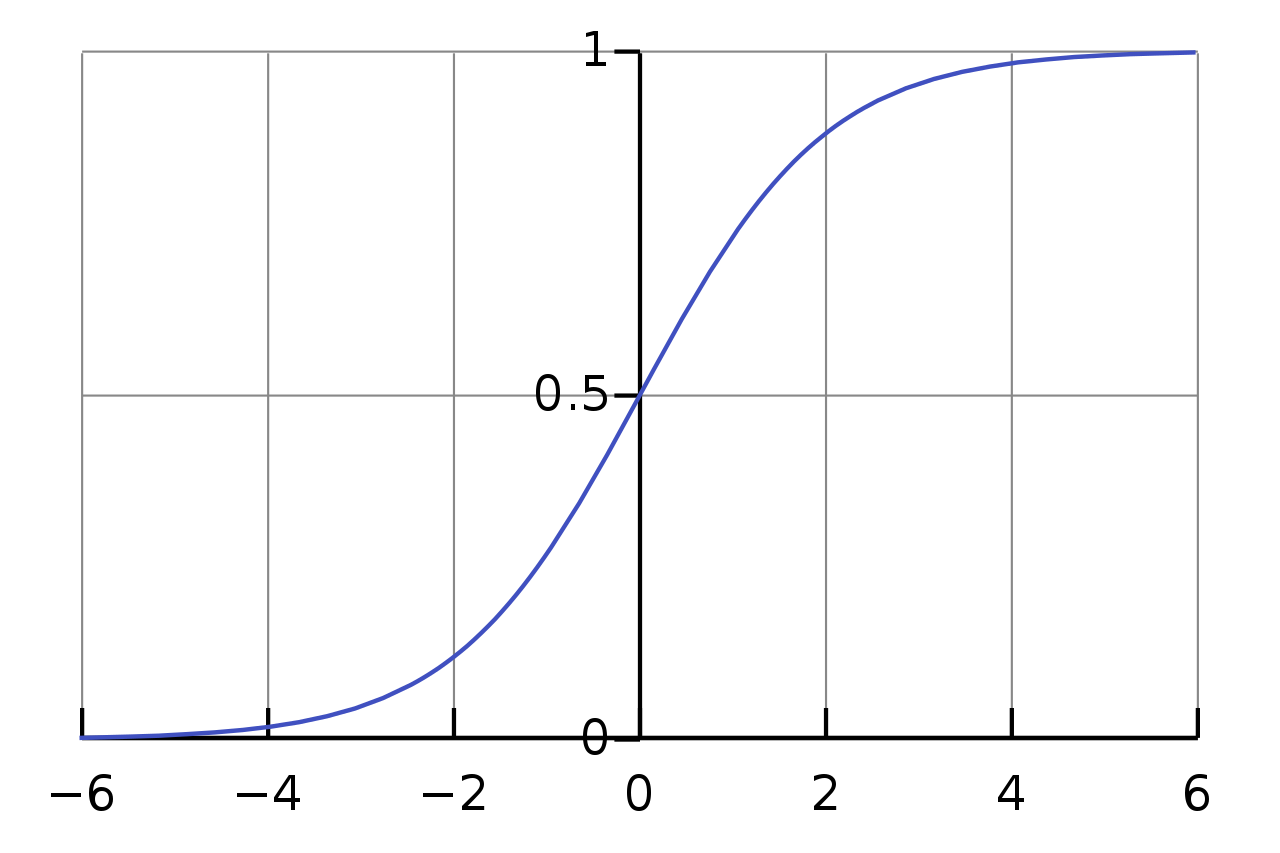
\includegraphics[scale=0.25]{NN/Logistic-curve}
	\centering
	\caption{Logistická funkce s~předpisem \eqref{eq:sigmoid}, zdroj: \parencite{wiki_logistic_function}}
	\label{fig:sigmoid}
	\end{figure}
	
	\subsubsection{Aktivační funkce}
	K~tomuto účelu se mohou využívat a v~praxi se využívají i jiné funkce. Obecně se jim říká aktivační funkce nebo také přenosové funkce \eqref{eq:f-aktivacni}. Je-li to skoková funkce s~pevnou hranicí (prahem), nazývá se neuron perceptron. V~případě, že se používá logistická funkce, setkáváme se často s~názvem sigmodiální perceptron. Logistické funkce mají výhodu v~tom, že jsou diferencovatelné. \parencite[\gls{str} 728-729]{AIAMA}, \parencite[\gls{str} 36]{NN_introduction-Kriessel}\\
	\begin{align}
	\label{eq:f-aktivacni}
	& a_j = g\left(\sum_{i=1}^{n} w_{i,j} a_i\right) && \text{kde $g()$ je aktivnační funkce}
	\end{align}
	Kromě \emph{Heavisideovy funkce} \parencite{wiki:H-funkce} \eqref{eq:H-funkce}, ta odpovídá normálnímu perceptronu, a logistické \ref{eq:sigmoid}, také občas nazývané jako Fermiho funkce, se využívá třeba i hyperbolický tangens(podobný průběh jako logistická funkce). \parencite[\gls{str} 37-38]{NN_introduction-Kriessel}
	\begin{equation}
	\label{eq:H-funkce}
	 H_p = 
		\begin{cases}
		0 & \text{pokud $x<0$}\\
		p & \text{pokud $x=0$}\\
		1 & \text{pokud $x>0$}
		\end{cases}
	\end{equation}
	\subsection{Topologie \gls{NS}}
	\label{sec:NN-topo}
	Existuje mnoho způsobů, jak neurony spojit ve funkční síť  \parencite{NN-zoo}. Nejzákladnější rozdělení je na \emph{dopředné \gls{NS}} (\gls{en} \emph{feed-forward networks}) a na \emph{rekurentní sítě}, kde neurony svými výstupy ovlivňují sebe (buď přímo, nebo ovlivní neuron, který poté ovlivňuje jej). Z~toho vyplývá, že odpověď této \gls{NS} záleží na počátečním stavu. Jedná se o~dynamický systém, který se nemusí ustálit a může oscilovat, či se chovat chaoticky. Dále mohou mít krátkodobou paměť (na rozdíl od \gls{FFN}). To je dělá zajímavějšími, ale také složitějšími. \parencite[\gls{str} 729]{AIAMA}\\
	\subsubsection{Dopředné neuronové sítě (\gls{FFN})}
	\label{sec:NN-FFN} 
	\Gls{en} nazývané \emph{Feed forward networks}, do češtiny by se dalo přeložit jako dopředné neuronové sítě. Síť je uspořádána do \emph{vrstev}. Jedna vstupní vrstva, jedna výstupní vrstva a mezi nimi nějaký počet skrytých vrstev. Výstupní spojení neuronů jdou vždy pouze do další vrstvy. Stejně tak vstupní spojení jsou vždy jen z~vrstvy předchozí. Neurony v~rámci jedné vrstvy nejsou propojené. Sítě, kde je každý neuron spojen s~každým neuronem z~další vrstvy nazýváme \emph{kompletně propojené}. V~některých případech zahrnují i \gls{tzv} zkratkové spojení, které přeskakují jednu nebo více vrstev, ale stále splňují podmínku, že směřují od vstupní vrstvy k~vrstvě výstupní. \parencite[\gls{str} 39-40]{NN_introduction-Kriessel}\\
	
	\subsection{Učení \gls{NS}}
	Učení nebo trénink \gls{NS} spočívá v~upravování sítě, tak aby její končená verze byla schopná dávat správné výstupy pro problémy nějaké kategorie s~přesností a obecností, jaká se po ní vyžadována. Výstup \gls{NS} může být změněn různými způsoby \parencite[\gls{s} 51]{NN_introduction-Kriessel}:
	\begin{enumerate}
	\item{Přidáním nebo odebráním spojení}
	\item{Změnou váhy existujícího spojení}
	\item{Změnou aktivačního prahu neuronu}
	\item{Změnou funkce uvnitř neuronu}
	\item{Přidáním a odebráním neuronu (a jeho spojení)}
	\end{enumerate}
	Nejběžnějším způsobem je změna hodnot vah a prahu. Navíc v~kompletně propojených sítích si můžeme představit odebrání spojení jen jako nastavení jeho váhy na nulu a přidání spojení jako opak. Změna vnitřní funkce je obtížná na implementaci, neintuitivní a nemáme motivující biologický vzor. Oproti tomu velký zájem se zaměřuje na přidávání a odebírání neuronů, protože to mění samotnou topologii \gls{NS} tak, aby byla lépe přizpůsobená konkrétnímu problému. Používá se \emph{evolučních postupů} (nebo algoritmů, \gls{viz} \ref{sec:genetic}), ve kterých podle zvolených mechanismů síť zmutuje několika způsoby a potom se vyberou ty nejvhodnější (\gls{tj} ty která mají výstupy/výsledky nejbližší ideálním). Z~toho vyplývá jejich nevýhoda, větší časová náročnost než u~přímých metod učení jako \emph{backpropagation}. \parencite[\gls{s} 52,127]{NN_introduction-Kriessel}\\
	
	\subsubsection{Backpropagation}
	\label{sec:BP}
	Používá se především ve vícevrstvých \gls{FFN}. \emph{Účelová funkce} (také cílová, kriteriální, nákladová \gls{en} \emph{objective} nebo také \emph{cost}, loss případně error function) \parencite[\gls{s} 77]{NN_introduction-Kriessel} \parencite[\gls{s} 733]{AIAMA} \parencite{wiki:ucelova-funkce} \parencite[\gls{k} 1.5]{NN-Nielsen-web} je funkce, která hodnotí výstup \gls{NS} (porovnává ho se správným výstupem). Jejího minima (nebo maxima podle definice, ale většinou se v~terminologii  používá minimalizace výstupní chyby) se snažíme dosáhnout. Jako vstup této funkce máme všechny váhy a prahy jako výstup. Spočítat globální minimum je velmi obtížné obzvláště pro takto komplikované funkce, ale je možné (a snadnější) spočítat její sklon. Budeme-li měnit váhy podle tohoto sklonu dosáhneme po několika opakováních lokálního minima, tento proces se nazývá \gls{en} \emph{gradient descent} (česky metoda sestupného gradientu(sklonu)).\parencite{3B1B-ch2}\\
	Existuje způsob, jak tento proces zapsat matematicky přes derivace \footcite[Anglicky s~pěkným grafickým znázorněním to popisuje Backpropagation calculus | Deep learning, chapter 4 od 3Blue1Brown na stránce YouTube]{3B1B-ch4}. Ale pro základní pochopení stačí následovně. Zadáme \gls{NS} jeden problém a výstup výstupních neuronů porovnáme s~ideálním výstupem. Čím větší rozdíl tím více je potřeba ho změnit, měníme tedy úměrně chybě. Výstup neuronu změníme změněním vah spojení z~předchozí vrstvy, ty měníme úměrně k~velikosti výstupu neuronu z~předchozí vrstvy. Dalším krokem je změnit výstupy neuronů z~předchozí vrstvy, ale tady mohou mít různé neurony výstupní vrstvy protichůdné zájmy. Ne každý zájem je stejně důležitý, takže se započítávají úměrně k~váze spojení mezi těmito neurony a úměrně velikosti chyby výstupního neuronu. Výsledná požadovaná změnu výstupu neuronů v~této vrstvě je tedy součtem všech zájmů z~předchozí vrstvy. Výstup ale nemůžeme měnit přímo, protože je závislý na neuronech z~vrstvy předchozí a vahách jejich spojení. To je ale v~podstatě stejný problém, jaký jsme řešili ve vrstvě předchozí, takže stačí zopakovat tento proces v~této vrstvě a pak v~následující a tak dále dokud nedosáhneme vrstvy vstupních neuronů. Odtud pochází název backpropagation, což se dá přeložit jako šíření zpět. Tohle je pouze pro jeden problém ve skutečnosti musíme vyzkoušet sadu problémů  a provést změnu nebo změny (\gls{viz} dělení na online a offline učení \doubleref{sec:on-off-lol}) \parencite{3B1B-ch3}
	
	\section{Fuzzy logika}
	\label{sec:fuzzy}
	Logika se zabývá formálními principy uvažování a odůvodňování. Fuzzy logika (z~angličtiny překládáno také jako mlhavá logika \parencite{wiki_fuzzy}) je zaměřena na přibližné odůvodňování. Buduje modely, které (podobně jako lidské uvažování) jsou schopny činit racionální rozhodnutí v~prostředí s~nepřesnými a nejasnými informacemi. \parencite[\gls{s} 83]{fuzzy_logic}
	\subsubsection{Lingvistická proměnná}
Je pojem ve fuzzy logice, který je klíčový při její aplikaci. Hodnoty jsou slova, slovní spojení nebo věty v~přirozeném nebo umělém jazyce. \Gls{napr} proměnná "věk" může nabývat hodnot: "mladý", "starý", "velmi mladý", "velmi starý", "ne mladý", "ne starý"  \gls{atd} Každá hodnota lingvistické proměnné reprezentuje rozdělení možností, \gls{viz} obrázek \ref{fig:linguistic_function}. \parencite[\gls{s} 90]{fuzzy_logic}, \parencite[\gls{str} 50]{soft_fuzzy}
\begin{figure}[h]
	\centering
	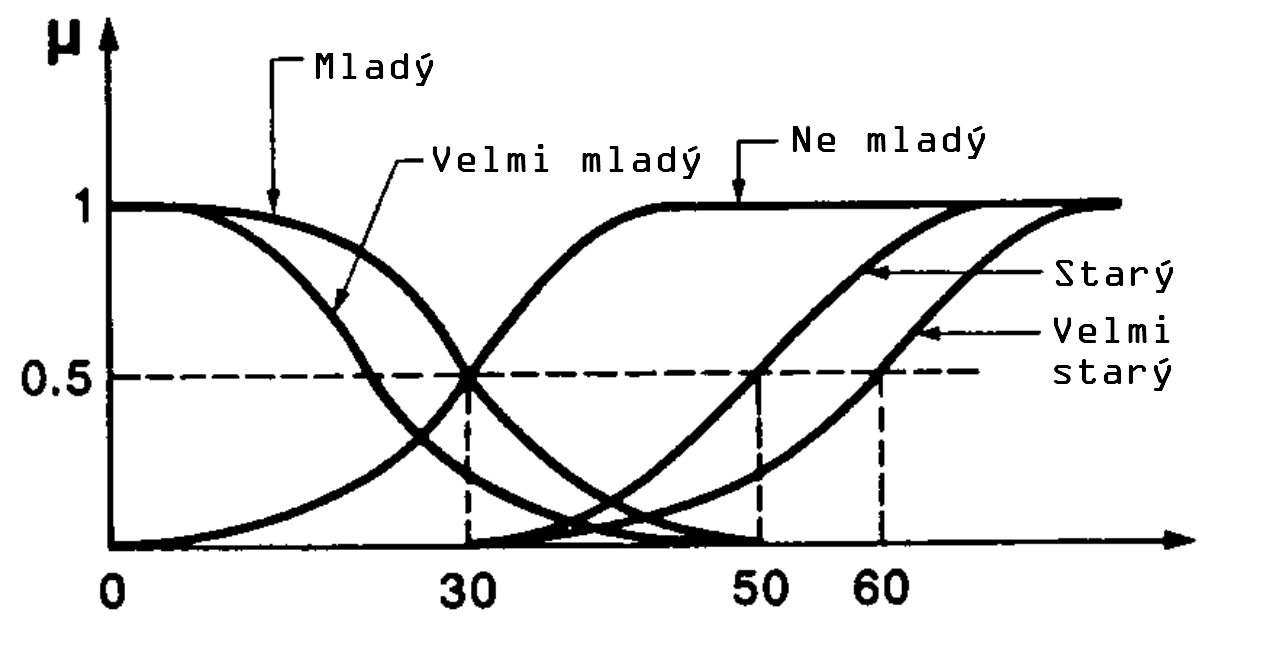
\includegraphics[scale=0.35]{NN/fuzzy_linguistic_function}
	\caption{Příklad rozdělení pravděpodobností u~lingvistické proměnné "věk", zdroj: \parencite[\gls{str} 90]{fuzzy_logic}, upraveno}
	\label{fig:linguistic_function}
	\end{figure}

	\section{Genetické algoritmy}	
	\label{sec:genetic} 
	\GLS{GA} patří do širší skupiny \emph{evolučních algoritmů}. Jsou to algoritmy inspirovány přírodní evolucí. \GLS{GA} jsou jednoduché na implementaci, ale jejich chování je často nepředvídatelné. Často se jim daří uspět v~praktických problémech. Máme mnoho různých kandidátních řešení (nazývaných jedinci nebo \emph{fenotypy}). Každé kandidátní řešení má své vlastnosti neboli chromosomy. Na začátku se náhodně vygeneruje populace. V~každé generaci se ohodnotí vhodnost jednotlivých řešení a ta nejlepší přežijí a do další generace postoupí jejich chromozomy, které se předtím mohou kombinovat a nebo náhodně mutovat. Tento postup je opakován. Ukončí se ručně nebo je-li dosaženo alespoň jedné z~podmínek  \parencite[\gls{str} 50-53]{chaudhuri2017optical} :
	\begin{enumerate}
	\item{Dosažený předem určený počet generací.}
	\item{Jsou vyčerpány zdroje (výpočetní nebo peněžní) pro pokračování.}
	\item{Výsledky se dalšími generacemi nezlepšují a nebo jsme dosáhli minimální kritéria.}
	\end{enumerate}
	Pro implementaci vyžadují \parencite[\gls{str} 50-53]{chaudhuri2017optical}:
	\begin{itemize}
	\item{Reprezentaci kandidátního řešení: typicky binární řetězec 1 a 0, ale jsou možné i jiné způsoby.}
	\item{Funkci vhodnosti (\gls{en} \emph{fitness function}, typ účelové funkce (více o~ní \ref{sec:BP} u~backpropagace)): určující, jak úspěšné je řešení}
	\end{itemize}





	
	
	\section{Možnosti dnešní \gls{AI}}
	\label{sec:AI-now} %state of the art
	
	\subsection{DeepMind}
	\label{sec:DeepMind}
	AlphaGo byla první \gls{AI}, která překonala světové šampióny stolní hry Go (populární v~Asii). Hluboké neuronové sítě vybírali tahy z~vyhledávacího stromu (\gls{en} tree search). Tyto sítě byly trénované pomocí tahů lidských profesionálů a hraním sami se sebou. Následovná \gls{AI}, AlphaGo Zero, byla trénovaná pouze pomocí reinforcement learning a hraním se sebou (\gls{en} \emph{self-play}) bez jakéhokoliv lidského vzoru. Toto vyústilo v~lepší herní schopnosti a tato \gls{AI} byla schopná porazit předchozí verzi 100-0. \parencite{AlphaGoZero} Dalším krokem bylo zobecnění tohoto postupu vznikla \gls{AI} \emph{AlphaZero}. Algoritmus, který je schopný se takto naučit několik her (šachy, Go, shogi) a získat přesvědčivě dobré výsledky nad nejlepšími algoritmy či umělými inteligencemi.\parencite{AlphaZero}\\
	Další hrou, na kterou se v~DeepMind zaměřili, byl StarCraft II. Je tomu z~podobných důvodů jako OpenAI a Dota 2. Učení hrou \gls{AI} se sebou samotnou muselo být trochu upraveno a připraveno, protože ve hře je velké množství strategií (množství různých typů jednotek a jejich kombinací) a proti-strategií (zjednodušeně kámen-nůžky-papír). Je totiž nutné zajistit, aby nedošlo k~tomu, že síť naučí hrát jednu dominantní strategii a jakmile nějaká verze nalezne proti-strategii, tak začne vyhrávat, až se z~této stane dominantní strategie, která zase přestane dominovat, až k~ní bude nalezena proti-strategie. Tím by \gls{AI} mohla ztratit "paměť", jak hrát proti jiným strategiím, než té dominantní.\parencite{AlphaStar}
	\subsection{OpenAI}
	\label{sec:OpenAI}
	OpenAI Five využívá deep reinforcement learning (\gls{viz} \doubleref{sec:AI-deleni}) na překonání nejlepších hráčů hry \emph{Dota 2}. Tato videohra je strategie v~reálném čase pro více hráčů, kde 2 týmy se základnami v~rozích čtvercové mapy soupeří, kdo zničí základnu nepřítele jako první. Byla zvolena, protože k~jejímu zdolání je nutné překonat řadu obtížně překonatelných problémů pro reinforcement learning, které jsou podobné těm, kterým čelí \gls{AI} v~reálném světě.
	\begin{itemize}
	\item Plánování do daleké budoucnosti: hra trvá běžně 45 minut a běží 30 snímku za vteřinu. To je i s~omezeným počtem akcí za vteřinu (OpenAI může provést akci každé 4 snímky) mnohonásobně víc než šachy nebo Go.
	\item Obrovské množství možných akcí a obrovské množství pozorovaných hodnot
	\item Každý tým (tedy i \gls{AI}) má neúplné informace o~přesném stavu hry. Vidí jen okolí spoluhráčů, jednotek a budov. Musí tedy předpokládat soupeřovo chování a strategii.
	\end{itemize}
	Rozšířením jíž existujících technik reinforcement učení, kde výrazně zvětšili měřítko. OpenAI Five se učilo hraním proti sobě v~rychlosti  zhruba 2 miliony snímků za 2 vteřiny. Nakonec zvládlo 17 (ze 117) hrdinů a porazilo v~roce 2019 ve hře  Dota 2 světové šampiony. Tím dokázalo, že i takto obtížné úkoly je možné zvládnout, máte-li dost velký výpočetní výkon, pomocí reiforcement učení. \parencite{openai2019dota}
\subsection{FAIR}
	\label{sec:FAIR}
	FAIR (\emph{Facebook Artificial Intelligence Research}) vytvořil \gls{AI} jménem \emph{Pluribus} (na základě \gls{AI} Libratus, které porazilo profesionální hráče pokeru ve hře jeden proti jednomu.). Tato \gls{AI} dokázala porážet profesionální hráče ve hře šesti hráčů. Zajímavé je tím, že se nejedná o~typickou 1v1 situaci, kdy jeden hráč prohraje a druhý vyhraje. Navíc poker je hra s~se velkým množstvím skrytých informací. Tohoto úspěchu bylo dosaženo opět využitím hry s~sebou samým (\gls{en} self-play) pomocí reinforcement learning. \parencite{FAIR-poker}
		
	
	\part{Praktická část}
	\chapter{Postup}
	Cílem praktické části je vytvořit program schopný rozpoznávat znaky, využijeme k~tomu \emph{Tesseract} (\gls{viz} \ref{sec:Tesseract}). Ten ale většinu věcí dělá už automaticky vnitřně, takže hlavním cílem bude upravit obrázek pomocí knihovny \emph{OpenCV} (\gls{viz} \ref{sec:OpenCV}, tak aby Tesseract byl schopný lépe rozeznávat znaky.
	
	\section{Použité nástroje}
	\label{sec:used}
	\subsection{Tesseract}
	\label{sec:Tesseract}
	Tesseract je \gls{OCR} nástroj psaný v~programovacím jazyce C++ (původně v~C).  Začínal v~polovině devadesátých let minulého století v~laboratořích Hewlett-Packard. V~roce 2005 společnost HP otevřela (\gls{tj} veřejně zpřístupnila) jeho zdrojový kód, a tak se Tesseract stal \gls{tzv} open source software. Následujícího roku se vývoje Tesseractu ujal Google. Nejnovější verze 4.0.0. podporuje \gls{utf-8} a dokáže rovnou po instalaci rozeznat více než 100 jazyků. Navíc může být trénován a naučit se rozeznávat i další jazyky. Pracuje se s~ním pomocí příkazové řádky, ale díky tomu, že se jedná o~projekt s~otevřeným zdrojovým kódem, existují grafická rozhraní vyvinutá třetími stranami. V~mnoha případech je možné zlepšit úspěšnost rozeznání tímto OCR, pokud je zlepšena kvalita obrázku. \parencite{tesseract_wiki}
	\subsubsection{Pytesseract}
	\label{sec:pytesseract}
	Pytessearact je nástroj, který umožňuje využívat Tesseract pomocí Pythonu. V~podstatě jen volá Tesseract přes příkazovou řádku. \parencite{pytesseract}
	\subsection{OpenCV}
	\label{sec:OpenCV}	
	OpenCV (\gls{en} \emph{Open Source Computer Vision Library}, v~češtině knihovna počítačového vidění s~otevřeným zdrojovým kódem) \parencite{opencv_library} obsahuje algoritmy jak pro počítačové vidění, tak i pro strojové učení. OpenCV je psané v~C++ a má rozhraní i v~Javě, Pythonu a MATLABu. Uplatněno je \gls{napr} ve sledování těžícího vybavení nebo v~kontrole, že se nikdo netopí v~bazénu. Je využíváno i známými společnostmi jako je Google, Microsoft a Intel. \parencite{opencv_about}
	\subsection{Datová sada}
	\label{sec:DataSet}
	K~otestování  využijeme \emph{Brno Mobile OCR Dataset} (\gls{zkr} \emph{\gls{B-MOD}}), protože obsahuje velké množství dat se správnými výsledky a s~různou úrovní obtížnosti. Vytištěné vědecké články byly foceny různými zařízeními v~nijak neomezených podmínkách, takže jsou různě rozmazané, nasvícené, \gls{atd} Jedna část je více než 500~000 řádek textu (každá jako samostatný obrázkový soubor) a mají přesné transkripce toho, co je na nich napsáno, takže můžeme snadno ověřit kvalitu našeho \gls{OCR} systému.  Tato část je dále rozdělena na 3 podmnožiny. Jsou to testovací, trénovací a ověřovací a všechny jsou ve třech úrovních obtížnosti: lehké, střední a těžké. \parencite{pero_dataset}, \parencite{BMOD_article}\\
	V~této práci budu využívat nějakou menší (z~důvodu délky výpočtu a také velikosti místa na disku) podmnožinu lehké obtížnosti, protože ta obsahuje dostatečný rozptyl náročnosti. Kromě jednoduchých obrázků se v~ní vyskytují i více či méně rozmazané řádky.
	\section{Způsoby úpravy obrázků}
	Samotná dokumentace Tesseractu doporučuje provést úpravu obrázku a uvádí rovnou několik příkladů.  \parencite{Tess_wiki_improve}
	\subsection{Grayscale a binarizace}
	 Jako první se nabízí převedení barevného obrázku do stupňů šedi (\gls{en} grayscale) nebo přímo jeho binarizace, která rozdělí všechny pixely obrázku buď na černé nebo bílé. Má 2 hlavní kategorie:
	 \begin{enumerate}
	 \item{\emph{Jednoduchý práh}: V~rámci celého obrázku, je jednotný (globální) práh, který určí, jestli bude pixel bílý nebo černý.}
	 \item{\emph{Adaptivní práh}:  Lokální práh se upravuje podle okolí, takže různé oblasti mají různý práh. To se hodí zejména pokud je nasvícení nerovnoměrné.}
	  \end{enumerate}
	 První přístup fungoval dostatečně dobře pro některé obrázky, ale jeden pevný práh pro celou sadu rozhodně nefungoval, protože některé málo nasvícené skončili celé černé a naopak ty přesvícené (nebo jen s~nevýrazným textem) skončili celé bílé. Proto je nutné využít nějaký z~adaptivních přístupů. To ale také není dostatečné, protože pozadí nemusí mít jednotnou barvu, ale může mít šum (některé pixely světlejší a jiné zase tmavší). Při binarizaci tak může dojít k~vytvoření tmavých teček či skvrn na pozadí (\gls{viz} \ref{fig:binarizace}) a ty by mohli být mylně považovány za znaky nebo jejich části Tesseractem.
	\begin{figure}
	 
\includegraphics[scale=0.8]{praxe/prah-nekvalitni}
	\centering
	\caption{Ilustrační obrázek binarizace: lines-42(15,2)-}
	\label{fig:binarizace}
	\end{figure}
	\subsection{Rozmazání}
	To nás vede k~rozmazávání (\gls{en} blurring), protože to by mohlo rozmazat pozadí a zmenšit tak rozdíly mezi jednotlivými pixely. Tím by se stalo pozadí více homogenním. Na druhou stranu by to mohlo rozmazat i znaky a zhoršit tak jejich rozpoznávání. Při rozmazávání se využívá například průměrování okolních hodnot nebo jejich střední hodnota.
	\subsection{Odstranění šumu}
	V~OpenCV se nachází i speciální funkce pro odstranění šumu z~fotografií, která je ale vnitřně složitější a vyžaduje více času pro výpočet.
	\subsection{Změna velikosti}
	Protože binarizací ztrácíme informaci (místo spousty úrovní šedi, máme jen 2 úrovně) a protože obrázky některé obrázky jsou s~malým rozlišením, může dojít ke ztrátě detailu, který může být nezbytně nutný k~rozeznání znaku. Tomuto bychom mohli částečně zabránit zvětšením obrázku. \Gls{napr} jeden šedý pixel se při binarizaci musí stát buď černým nebo bílým, ale pokud místo něj budeme mít 4 šedé pixely, tak se 2 mohou stát bílými a 2 černými a zachovat tím přesněji předchozí stav.
	\section{Automatizace}
	K~nalezení správné kombinace takových funkcí a jejich parametrů, aby se zlepšila rozpoznávací schopnost Tesseractu, je třeba vytvořit si nějaký systém. Musí být schopen vytvořit a porovnat velké množství způsobů úpravy obrázku, pokud možno s~minimálním zapojením člověka, aby mohl program běžet delší dobu sám, \gls{napr} přes noc.
	\begin{enumerate}
	\item{\emph{mastercv.py}: Používá OpenCV a podle předloženého textového souboru provede úpravu obrázků a uloží je systematicky do složek.}
	\item{\emph{tesseract.py}: Předložený textový soubor obsahuje seznam složek a seznam obrázků v~nich. Program provede \gls{OCR} a výsledek uloží do textového souboru pojmenovaného podle názvu obrázku. }
	\item{\emph{accuracy.py}: Podle seznamu složek a seznamu obrázků, ve kterém jsou přiloženy i správné odpovědi, provede výpočet úspěšnosti Tesseractu.}
	\end{enumerate}
	Jako první je třeba znát formát \gls{B-MOD}, aby jsme s~ním mohli pracovat. Ve složce se nachází textové soubory(rozdělené podle obtížnosti a typu), které mají na každé řádce unikátní název obrázku a (kromě testovacích sad) mezerou oddělený textový řetězec, který je správným řešením. Dále je tam jen složka se všemi obrázky. Protože jsou všechny sady zbytečně velké pro naše účely, tak si jednoduše část (zhruba 2000 řádek) jedné lehké vykopírujeme do vlastního souboru \emph{small.easy}, který budeme využívat jako databázi.
	\subsection{mastercv.py}
	Následuje příkazy ze souboru \emph{prikazy-pro-opencv.txt}. Ten obsahuje mezerou oddělené informace. První je zdrojová složka, ze které má brát obrázky. Druhá je databáze (neboli seznam) obrázků, v~našem případě je to \emph{small.easy}. Jako třetí je název souboru, ze kterého má brát parametry pro jednotlivé funkce (\gls{napr} \emph{parametry1.txt}). V~souboru s~parametry jsou údaje na jedné řádce a od sebe oddělené mezerou. A pak následují mezerou oddělené číselné kódy pro funkce knihovny openCV. Tyto kódy jen reprezentují, jaká funkce se mají vykonat (\gls{viz} \ref{sec:docs})
	\subsubsection{Proces}
	\begin{enumerate}
	\item{Otevři soubor s~příkazy a pro každou řádku opakuj:}
	\item{Vyzkoušej funkčnost parametrů a ulož si je.}
	\item{Vyzkoušej, jestli všechny kódy příkazů odpovídají nějakým příkazům. A přitom vytvoř systematický název cílové složky.}
	\item{Vyzkoušej, jestli existuje složka se zdrojovými obrázky.}
	\item{Jestli vše sedí pokračuj, jestli ne přeskoč řádku.}
	\item{Vytvoř cílovou složku se systematickým názvem, jestli neexistuje.}
	\item{Jestli existuje soubor s~databází obrázků, pokračuj. Jinak přeskoč řádku.}
	\item{Pro každý řádek v~databázi obrázků opakuj:}
	\item{Otevři obrázek ze zdrojové složky.}
	\item{Proveď každý příkaz ze seznamu příkazů.}
	\item{Ulož obrázek do cílové složky.}
	\item{Pokračuj na další řádek v~databázi obrázků.}
	\item{Po dokončení celé databáze, pokračuj na další řádek příkazů.}
	\end{enumerate}	
	
	\subsubsection{Dokumentace kódů funkcí}
	\label{sec:docs}
	\begin{outline}
\1 \emph{0} : obrazek = cv2.resize(obrazek, None, fx=\emph{par0}, fy=\emph{par0}, \\interpolation=\emph{interpolace})\\
	$fx$ a $fy$ násobí velikost původního obrázku a získávají tak velikost výsledného obrázku. Přísluší jednotlivým osám. Jedná se o~desetinná čísla. \parencite{CV_resize}
	\2 \emph{01}: $interpolace$ = cv2.INTER\_AREA\\ Vhodné pro zmenšování obrázku.
	
	\2 \emph{02}: \emph{interpolace} = cv2.INTER\_CUBIC\\ Nejlepší pro zvětšení obrázku, ale pomalejší.
	
	\2 \emph{03}: \emph{interpolace} = cv2.INTER\_LINEAR\\ Pro zvětšení obrázku. Rychlejší, ale ne nejlepší.  
	
\1 \emph{11}: obrazek = cv2.cvtColor(obrazek, cv2.COLOR\_BGR2GRAY)\\ Převede obrázek do grayscale.
\1 \emph{21}: obrazek = cv2.fastNlMeansDenoising(obrazek, $par1$,$par2$, $par3$)\\
Vyžaduje grayscale obrázek. Desetinné číslo $par1$ určuje sílu filtru. Celá lichá čísla $par2$ a $par3$ jsou parametry určující velikost okna. Výpočetní náročnost se zvětšuje pro vyšší hodnoty.
\1 \emph{3}: Provede rozmazání (\gls{en} blurring) obrázku. \parencite{CV_blur}
	\2 \emph{31}: obrazek = cv2.blur(obrazek, ($par4$, $par4$))\\ Použije aritmetický průměr pole, kde výška a šířka je rovna $par4$, což je celé číslo.
	\2 \emph{32}: obrazek = cv2.bilateralFilter(obrazek, $par5$,  $par6$, $par7$)\\
	Je efektivní pro odstranění šumu a zároveň zachovává ostré hrany. $par5$ je celé číslo určující průměr okolí použitého ve filtraci.	 $par6$ a $par7$ jsou desetinné hodnoty odpovídající SigmaSpace a SigmaColor. Čím jsou větší, tím větší je síla efektu (\gls{viz} dokumentace \parencite{CV_bilateral}
	\2 \emph{33}: obrazek = cv2.GaussianBlur(obrazek, ($par8$,$par8$), $par9$)\\  $par8$ určuje velikost oblasti, se kterou se počítá, musí být kladné liché číslo. $par9$ určuje standartní deviaci, pokud je nulový, tak se vypočítá z~velikosti oblasti
	\2 \emph{34}: obrazek = cv2.medianBlur(obrazek, $par10$) \\ Střed pole o~výšce a šířce $par10$ je určen mediánem hodnot v~tomto poli. $par10$ by měl být kladná liché číslo.
\1 \emph{4} Vstupem by měl být grayscale obrázek.  Výsledek je binarizovaný obrázek \parencite{CV_threshold}
	\2 \emph{41}: obrazek = cv2.adaptiveThreshold(obrazek, 255,\\cv2.ADAPTIVE\_THRESH\_MEAN\_C, cv2.THRESH\_BINARY, $par11$, $par12$)\\ Celé číslo $par11$ určuje velikost bloku. Spočítá se průměr a odečte se od něj konstanta $par12$.
	\2 \emph{42}:  obrazek = cv2.adaptiveThreshold(obrazek, 255,\\cv2.ADAPTIVE\_THRESH\_GAUSSIAN\_C, cv2.THRESH\_BINARY, $par13$, $par14$)\\ Celé číslo $par13$ určuje velikost bloku. Spočítá se průměr a odečte se od něj konstanta $par14$.
	\2 \emph{43}: ret, obrazek = cv2.threshold(obrazek, 0, 255, cv2.THRESH\_BINARY + cv2.THRESH\_OTSU)\\
	Jedná se o~binarizaci s~globálním prahem, který je určen pomocí Otsuovi metody. Nevyžaduje žádný parametr. Funkce vrací 2 hodnoty a až druhá je upravený obrázek.
\end{outline}
	\subsection{tesseract.py}
	Očekává ve vstupním souboru 2 informace oddělené mezerou na každé řádce. První je název složky, ze které má brát obrázky. Druhý je název textového souboru, ve kterém je uložen databáze názvů obrázků. Pak postupně každý obrázek předloží Tesseractu na rozpoznání a výsledek uloží do zdrojové složky do textového souboru, který nese stejný název jako obrázek plus koncovka '.tess'.\\
	V~některých případech Tesseract rozezná znaky, které není Python schopen uložit. V~tomto případě prostě uloží do souboru \textit{Encoding\_failed} a ztráta pár souborů, která tímto vznikne, je vzhledem k~velikosti našeho vzorku zanedbatelná.
	\subsection{accuracy.py}
	\subsubsection{Míra chybovosti ve slovech}
	Vypočítává zjednodušenou obdobu \emph{word error rate} (česky \emph{míra chybovosti ve slovech}). V~tomto případě je to počet slov, které \gls{OCR} nerozpoznalo, děleno počtem slov, které mělo rozpoznat. To znamená, že dostaneme číslo od 0 (ideální stav, kdy bylo vše rozpoznáno správně) do 1 (nejhorší stav, kdy nebylo rozpoznáno ani jedno slovo správně). To můžeme také převést do procent pro lepší čtení člověkem.\\
	V~praxi se obvykle počítá, kolika změnami (\gls{tj} přidání, odebrání nebo přepsání slova) se dosáhne cílového textu z~textu získaného pomocí \gls{OCR}. Tato hodnota se potom vydělí počtem slov ve vzoru.  Výsledná hodnota ale může být větší než jedna. \Gls{napr} když místo jednoho slova to nalezne 2 jiná, tak k~opravě textu jsou potřeba 2 operace, a proto je míra chybovosti rovna 2 (neboli 200\%). \parencite{wiki_wer}\\
	\subsubsection{Postup}
	 Předpokládá stejný formát jako \emph{tesseract.py}. Rozdělí cílový text podle mezer na jednotlivá slova. To samé provede pro text rozeznaný Tesseractem. A každé toto slovo porovnává s~cílovými slovy. Pokud se shodují, tak se toto cílové slovo odstraní. Toto pokračuje dokud to neprojde všechna přeložená slova, nebo dokud už nezbývají žádná cílová slova. Poté se porovná počet nenalezených cílových slov s~jejich původním počtem a tím zjistíme jakou část slov Tesseract nerozpoznal. Čím nižší, tím lepší výsledek.\\
	 \subsubsection{Nedostatky a problémy}
	Tento postup samozřejmě není úplně přesný, protože nebere v~potaz pořadí slov, takže může dojít k~falešně pozitivním shodám, ale toto hrozí jen pro velmi krátká slova, protože pravděpodobnost, že náhodou trefí  dlouhé slovo je minimální. Dále vůbec nerozlišuje mezitím, je-li ve slově chyba jednoho písmene, nebo je celé úplně špatně. Ale toto je snadno vykompenzováno dostatečně velkou sadou.\\	
	Dalším problémem je, že v~některých obrázcích, jsou částí sousedních řádek, které Tesseract správně identifikuje jako text, ale není schopen je rozeznat, takže vzniknou jen skupiny náhodných znaků, které se nám uloží na jiné řádky do souboru. Mohli bychom proto kontrolovat jen jednu řádku, ale protože nevíme kolikátá to je a navíc v~některých případech Tesseract rozdělí jednu řádku kvůli jemnému zahnutí textu na dvě, tak musíme nahradit konce řádků mezerami a tento výsledný text využít k~porovnání. Výpočetní čas je stejně velmi krátký (zejména oproti Tesseractu), takže je to minimální problém.\\
	\subsubsection{Tvar výstupu}
	Výsledek je uložen do textového souboru, kde každému řádku připadá jedna složka a tabulátory oddělené další informace. Tabulátory jsou zvoleny, aby šly výsledky snadno vykopírovat do tabulkového editoru. Z~hlediska dalšího zpracování Pythonem nebo jiným programem je stejně snadné rozdělit řádku podle tabulátorů jako podle mezer. Jako další informace je tam uložen poměr počtu nenalezených cílových slov a počtu všech cílových slov. \\Další informací je průměr tohoto poměru pro jednotlivé řádky. Tato informace není, tak důležité jako předchozí, protože neuvažuje  počet slov v~jednotlivých řádkách. Při dostatečně velkém vzorku, který má stejně reprezentované dlouhé a krátké řádky, by se tato hodnota měla přiblížit první. \\Jako další je opět první informace, ale tentokrát ve tvaru neusměrněného zlomku. A jako poslední je počet řádků, které byly využity. Z~tohoto čísla můžeme zjistit, kolik platných souborů zbylo po vyloučení těch, které vyhodili nějakou neočekávanou chybu (nejčastěji Tessearact nalezl neuložitelný znak). Můžeme tak zjistit reálnou velikost našeho vzorku.
\chapter{Výsledky měření}
	Nakonec bylo porovnáno zhruba 120 řádků příkazů, které byly puštěny na databázi asi 2~000 jmen obrázků. Přestože v~některých případech OpenCV vykonává operace zbytečně, tak běželo relativně rychle. Jediný trochu pomalejší příkaz je \emph{21} (odstranění šumu). Nejpomalejší částí je určitě Tesseract, kterému trvalo projet databázi o~cca 200~000 obrázcích asi 43 hodin (oproti asi 5-8 hodinám OpenCV). Závěrečné určení přesnosti trvalo sotva pár minut. Kompletní tabulka je k~nahlédnutí na konci maturitní práce \ref{table:komplet}.\\ 
	Výtah těch nejlepších postupů je v~tabulce \ref{table:nejlepsi}. Jak je vidět jen pár jich překonalo výsledek Tesseractu na neupravených obrázcích (\gls{tj} složka s~názvem \emph{lines-}). Úplně nejlepšího výsledku dosáhlo změnění velikosti obrázku na 4 násobnou. To může souviset s~tím, že Tesseract má z~nějakého důvodu optimální velikost písma, při které podává nejlepší výkon (podrobnosti  \gls{viz} \parencite{tess_weird}). Překvapivě další úprava už výsledek jen zhoršovala i v~případě, kdy se jednalo pouze o~převedení do grayscale (\gls{tj} složka s~názvem \emph{lines-02(04)-11-}). Dalším neúspěchem byla funkce na odstranění šumu a také všechny binarizační funkce. V~podstatě vždy, když byly použity, tak došlo ke zhoršení výsledků.\\ 
	Cíl naší práce jsme splnili a dokázali jsme najít takové úpravy, které zlepšují výsledky \gls{OCR}. Nejlepší úprava (\gls{tj} 4 násobné zvětšení obrázku) nám zajistila počet rozeznaných větší slov o~$0.86\%$. Další úspěšné kombinace už upravovali zvětšený obrázek, takže ve skutečnosti oproti předchozímu stavu výsledek zhoršovali. Jednou z~nich je \emph{31} (\gls{tj} rozmazání využívající aritmetického průměru pole), která překonala původní obrázky s~2 různými parametry (5 a 7). Můžeme vidět klesající tendenci s~klesající hodnotou parametru, takže je možné, že lze dosáhnout ještě lepších výsledků pomocí této funkce, pokud zmenšíme parametr, a možná i překonat \emph{lines-02(4)- }.\\
	Další kombinací, která překonala původní obrázky je bilaterální rozmazávání (\emph{lines-02(4)-11-32(7,60,60)-}). Protože tato funkce má 3 parametry, je těžké předpokládat, jestli (a případně jaká) je nějaká jejich kombinace lepší. Jediný způsob je prostě vyzkoušet několik možností a změřit výsledky a zjistit, jestli je vidět nějaká tendence.\\
	Dále jsme našli množství úprav, které naopak výsledky zhoršují. Takže pokud chceme úpravou obrázku zajistit lepší výsledky, je třeba zvolit správné funkce a najít ty správné parametry, aby jsme vůbec měli šanci na zlepšení. V~případě, že výběr neuděláme pořádně, tak si naopak pravděpodobně výsledky Tesseractu ještě zhoršíme, a pokud jsme neopatrní , tak můžeme i opravdu výrazně (\gls{viz} konec tabulky \ref{table:komplet}).
\begin{table}[h]
\begin{tabular}{|l|l|l|}
\hline
Název složky                & Nerozpoznaných slov  v~\% & Průměrný řádek v~\% \\ \hline
lines-02(4)-                 & 28.48375654523957         & 31.147177841597875 \\ \hline
lines-02(4)-11-31(5,5)-     & 28.772635814889334        & 31.44496288610835  \\ \hline
lines-02(4)-11-31(7,7)-     & 29.146799798059124        & 31.813984765368506 \\ \hline
lines-02(4)-11-32(7,60,60)- & 29.190832817163127        & 31.78324795699035  \\ \hline
lines-02(4)-11-             & 29.212795549374132        & 31.81483729252857  \\ \hline
lines-                      & 29.342969051690847        & 31.873574800141737 \\ \hline
lines-11- & 29.363382135219606 & 31.760516223353818 \\ \hline
lines-02(4)-11-32(9,75,75)- & 29.42031415953938         & 32.124600424025984 \\ \hline
lines-02(4)-11-33(7,7,7)-  & 29.59177943736313         & 32.18702065357416  \\ \hline
lines-02(4)-11-31(9,9)-     & 29.606325519238265        & 32.249597044580507 \\ \hline
lines-02(4)-11-32(5,90,90)- & 29.661776234740735        & 32.39996911754059  \\ \hline
lines-02(4)-11-33(9,9,9)-   & 29.69534650150653         & 32.396897053992784 \\ \hline
\end{tabular}
\caption{Nejlepší  seznamy příkazů}
\label{table:nejlepsi}
\end{table}
	
	\appendix
	\addcontentsline{toc}{part}{Apendix}
	\chapter*{Závěr}
	\addcontentsline{toc}{chapter}{Závěr}
	V~teoretické části jsou vysvětleny základní informace \gls{OCR} a \gls{AI}. Jsou zde popsány techniky optického rozpoznávání znaků. Skenování fyzického textu a úprava získaného obrázku jeho předzpracováním a následné rozdělení znaků, tak aby byly zachovány všechny důležité vlastnosti pro jejich rozeznání. V~části o~umělých inteligencích je kromě neuronových sítí popsána také mlhavá logika. \\
	V~praktické části jsem vytvořil systém na provedení velkého množství různých úprav obrázků pomocí OpenCV. Výsledné obrázky jsou potom předloženy Tesseractu, který zkusí rozeznat, co je na obrázku za text. A poslední část systému porovná úspěšnost Tesseractu na různě upravených obrázcích. \\
	Pomocí tohoto systému jsem zjistil, že je úpravou obrázků pomocí OpenCV možné zlepšit úspěšnost Tesseractu, protože jsem takovou úpravu našel. Jedná se o~zvětšení obrázku. Nalezl jsem i další kombinace úprav, které jsou lepší než původní obrázky, ale všechny vycházejí již ze zvětšených obrázků a oproti nim dochází ke zhoršení. Některé typy rozmazávání vykazovali potenciál, ke zlepšení oproti pouhému zvětšení obrázku při vhodné úpravě parametrů.\\
	 Přestože naměřené výsledky nemusí být obecně platné v~rozdílné sadě obrázků, tak vytvořený systém může být použit k~přiblížení se nejlepší kombinaci funkcí a jejich parametrů i pro jiné sady dat.\\
	 Na tuto práci lze navázat ještě větším zautomatizováním  a provázáním procesů tak, aby obrázky upravené OpenCV byly rovnou předány Tesseractu. Tím se ušetří místo na disku, což je důležité obzvláště při využívání větších datasetů a velkého množství kombinací příkazů OpenCV. Dále by mohl program sám z~naměřených hodnot určit, které úpravy jsou nejvýhodnější a u~nich systematicky zkoušet různé hodnoty parametrů tak, aby bylo nalezeny optimální příkazy, které umožní Tesseractu nejlepší rozpoznání.\\
	 Pro zájemce je celá práce a zdrojové kódy k dispozici na: \url{https://github.com/AmbryTheBlue/OCR-image-compraison}
	\nocite{*}
	
	
    \printbibliography					% Vytvoří seznam literatury
	\addcontentsline{toc}{chapter}{Bibliografie}
	
    \printglossary[title={Zkratky}]		% Vytvoří seznam zkratek
    \listoffigures				%Vytvoří seznam použitých obrázků
    \addcontentsline{toc}{chapter}{Seznam použitých obrázků} %přidá seznam použitých obrázků do obsahu
   
    \listoftables 		%Vytvoří seznam tabulek
    \addcontentsline{toc}{chapter}{Seznam tabulek}
    
	\lstlistoflistings
	\addcontentsline{toc}{chapter}{Seznam zdrojových kódů}
	
    
    \begin{prilohy}
    	\pitem{Kód programu}
    	\pitem{Tabulka všech naměřených hodnot}
    	\eitem{Vlastní program}
    	\eitem{Dokumentace}
    	\eitem{Část testovacích dat}  	
    \end{prilohy}
    
    \chapter{Přiložené soubory}
	\section{mastercv.py}
	\lstinputlisting[language=Python, basicstyle=\scriptsize , caption=mastercv.py]{mastercv.py}
	\section{tesseract.py}
	\lstinputlisting[language=Python, caption=tesseract.py, basicstyle=\scriptsize]{tesseract.py}
	\section{accuracy.py}
	\lstinputlisting[language=Python, basicstyle=\scriptsize , caption=accuracy.py]{accuracy.py}
	
\begin{landscape}
\section{Kompletní tabulka naměřených hodnot}

\begin{longtable}{ | p{5cm} | *{15}{c|}}
\hline
\multicolumn{1}{|l|}{Název složky}                & \multicolumn{1}{l|}{Poměr nerozpoznaných slov} & \multicolumn{1}{l|}{Průměrný řádek} & \multicolumn{1}{l|}{Poměr nerozpoznaných slov} & \multicolumn{1}{l|}{Počet řádků} \\ \hline
lines-02(4)-                                      & 0.2848375654523957  & 0.31147177841597873 & 5059/17761  & 1958 \\
lines-02(4)-11-31(5,5)-                           & 0.28772635814889336 & 0.3144496288610835  & 5148/17892  & 1970 \\
lines-02(4)-11-31(7,7)-                           & 0.29146799798059125 & 0.3181398476536851  & 5196/17827  & 1966 \\
lines-02(4)-11-32(7,60,60)-                       & 0.29190832817163126 & 0.3178324795699035  & 5184/17759  & 1962 \\
lines-02(4)-11-                                   & 0.2921279554937413  & 0.3181483729252857  & 5251/17975  & 1977 \\
lines-                                            & 0.2934296905169085  & 0.31873574800141735 & 5319/18127  & 1995 \\
lines-11- & 0.29363382135219606 & 0.31760516223353818 & 5355/18237 & 2003 \\
lines-02(4)-11-32(9,75,75)-                       & 0.2942031415953938  & 0.32124600424025984 & 5263/17889  & 1968 \\
lines-02(4)-11-33(7,7,7)-                        & 0.2959177943736313  & 0.3218702065357416  & 5270/17809  & 1963 \\
lines-02(4)-11-31(9,9)-                           & 0.29606325519238263 & 0.3224959704458051  & 5317/17959  & 1975 \\
lines-02(4)-11-32(5,90,90)-                       & 0.29661776234740733 & 0.3239996911754059  & 5297/17858  & 1967 \\
lines-02(4)-11-33(9,9,9)-                         & 0.2969534650150653  & 0.32396897053992785 & 5322/17922  & 1974 \\
lines-02(4)-11-34(9)-                             & 0.3009725111023666  & 0.326157390736683   & 5354/17789  & 1963 \\
lines-02(4)-11-34(11)-                            & 0.30341761600444567 & 0.33111919916946325 & 5460/17995  & 1979 \\
lines-02(4)-11-34(7)-                             & 0.30373230373230375 & 0.33316244704289033 & 5428/17871  & 1968 \\
lines-02(4)-11-33(11,11,11)-                       & 0.30629277249207143 & 0.3374442081132987  & 5505/17973  & 1981 \\
lines-02(4)-11-21(3,12,11)-                       & 0.31626912691269127 & 0.34203520576426194 & 5622/17776  & 1961 \\
lines-02(4)-11-21(2,17,7)-                        & 0.3277873932220423  & 0.35356024444515505 & 5871/17911  & 1971 \\
lines-02(4)-11-43-                                & 0.33463437033635635 & 0.35935778912735766 & 5830/17422  & 1927 \\
lines-02(4)-11-43-                                & 0.33463437033635635 & 0.35935778912735766 & 5830/17422  & 1927 \\
lines-02(4)-11-43-                                & 0.33463437033635635 & 0.35935778912735766 & 5830/17422  & 1927 \\
lines-02(4)-11-31(5,5)-43-                        & 0.3408173705451032  & 0.3643741739331804  & 5996/17593  & 1948 \\
lines-02(4)-11-33(7,7,7)-43-                     & 0.34364691161415084 & 0.3695983695298388  & 6042/17582  & 1948 \\
lines-02(4)-11-32(9,75,75)-43-                    & 0.3480196324620477  & 0.3717901792296982  & 6098/17522  & 1942 \\
lines-02(4)-11-34(7)-43-                          & 0.35752383113935543 & 0.38344194952776406 & 6301/17624  & 1946 \\
lines-02(4)-21(3,25,11)-11-                       & 0.3583393622349602  & 0.3877713976220303  & 6439/17969  & 1977 \\
lines-02(4)-11-21(3,25,11)-                       & 0.3592394929953302  & 0.38985381450112555 & 6462/17988  & 1979 \\
lines-02(4)-11-21(3,25,11)-32(5,90,90)-           & 0.3598510117856349  & 0.39169366422520757 & 6473/17988  & 1979 \\
lines-02(4)-11-21(3,25,11)-32(7,60,60)-           & 0.3623575201556853  & 0.392219112779942   & 6517/17985  & 1980 \\
lines-43-                                         & 0.36273380505731995 & 0.38578192584403126 & 6613/18231  & 2001 \\
lines-02(4)-11-21(5,27,7)-                        & 0.36282590412111015 & 0.3904459067605987  & 6471/17835  & 1968 \\
lines-02(4)-11-21(3,25,11)-33(7,7,7)-            & 0.36480543339085897 & 0.39420820806136136 & 6553/17963  & 1975 \\
lines-02(4)-11-21(3,25,11)-34(7)-                 & 0.36667959873635203 & 0.3948610633207491  & 6616/18043  & 1983 \\
lines-02(4)-11-21(3,25,11)-31(5,5)-               & 0.36764052432792715 & 0.397729864963413   & 6619/18004  & 1976 \\
lines-02(4)-11-21(3,25,11)-31(9,9)-               & 0.3685378300421566  & 0.39946384196700463 & 6644/18028  & 1983 \\
lines-02(4)-11-21(3,25,11)-31(7,7)-               & 0.3697652372720683  & 0.39885286724767144 & 6631/17933  & 1973 \\
lines-02(4)-11-21(3,25,11)-33(9,9,9)-             & 0.37304948729380294 & 0.40712522572066967 & 6694/17944  & 1978 \\
lines-02(4)-11-21(3,25,11)-34(9)-                 & 0.37392900856793143 & 0.40448577185817547 & 6721/17974  & 1973 \\
lines-02(4)-11-21(3,25,11)-32(9,75,75)-           & 0.37512537612838515 & 0.402608035180929   & 6732/17946  & 1977 \\
lines-02(4)-11-21(3,25,11)-34(11)-                & 0.38103457876273733 & 0.41043823164496784 & 6843/17959  & 1975 \\
lines-02(4)-11-21(3,25,11)-33(11,11,11)-           & 0.3816518847006652  & 0.41552696569581904 & 6885/18040  & 1982 \\
lines-02(4)-11-21(3,25,11)-31(5,5)-41(15,2)-      & 0.41113039167079823 & 0.42522427313352135 & 6634/16136  & 1801 \\
lines-02(4)-11-21(3,25,11)-34(7)-41(15,2)-        & 0.41169561723434506 & 0.42552277540171846 & 6660/16177  & 1803 \\
lines-02(4)-21(3,25,11)-11-33(7,7,7)-41(15,2)-   & 0.4121469632591852  & 0.4260183392627991  & 6596/16004  & 1792 \\
lines-02(4)-11-21(3,25,11)-41(15,2)-              & 0.41224565070387903 & 0.4259137147700568  & 6706/16267  & 1814 \\
lines-02(4)-11-21(3,25,11)-33(7,7,7)-41(15,2)-   & 0.4132451150136038  & 0.42485091039310285 & 6683/16172  & 1801 \\
lines-02(4)-21(3,25,11)-11-31(5,5)-41(15,2)-      & 0.4138524943101433  & 0.42905082571433706 & 6728/16257  & 1815 \\
lines-02(4)-21(3,25,11)-11-32(9,75,75)-41(15,2)-  & 0.417137245273754   & 0.4321916080717336  & 6796/16292  & 1820 \\
lines-02(4)-21(3,25,11)-11-34(7)-41(15,2)-        & 0.41845201238390095 & 0.430243213629288   & 6758/16150  & 1808 \\
lines-02(4)-11-21(3,25,11)-32(9,75,75)-41(15,2)-  & 0.41994330087513865 & 0.4357179392216863  & 6814/16226  & 1813 \\
lines-41(11,10)-                                  & 0.4204489053107594  & 0.43249906950247186 & 7624/18133  & 1993 \\
lines-02(4)-11-21(3,25,11)-32(5,90,90)-43-        & 0.4404662316658301  & 0.46839035184464806 & 7898/17931  & 1974 \\
lines-02(4)-21(3,25,11)-11-31(5,5)-43-            & 0.44207998212689903 & 0.46959230119364065 & 7915/17904  & 1970 \\
lines-02(4)-11-21(3,25,11)-31(7,7)-43-            & 0.4421187052356893  & 0.46831159695941316 & 7963/18011  & 1982 \\
lines-02(4)-11-21(3,25,11)-43-                    & 0.4427704070159658  & 0.4694409176977171  & 7876/17788  & 1961 \\
lines-02(4)-11-21(3,25,11)-43-                    & 0.4427704070159658  & 0.4694409176977171  & 7876/17788  & 1961 \\
lines-02(4)-11-21(3,25,11)-43-                    & 0.4427704070159658  & 0.4694409176977171  & 7876/17788  & 1961 \\
lines-02(4)-11-21(3,25,11)-31(5,5)-43-            & 0.4437363743082341  & 0.4724686059411151  & 7938/17889  & 1969 \\
lines-02(4)-11-21(3,25,11)-33(7,7,7)-43-         & 0.44596397598398935 & 0.47209662509524053 & 8022/17988  & 1979 \\
lines-02(4)-21(3,25,11)-11-33(7,7,7)-43-         & 0.44605878423513695 & 0.4727759656738389  & 8013/17964  & 1975 \\
lines-02(4)-11-21(3,25,11)-32(7,60,60)-43-        & 0.4485776805251641  & 0.47565068768498503 & 7995/17823  & 1964 \\
lines-21(3,12,11)-                                & 0.4507606964354369  & 0.47191104476346185 & 8207/18207  & 2000 \\
lines-02(4)-11-21(3,25,11)-32(9,75,75)-43-        & 0.4514727991536277  & 0.478378272696113   & 8108/17959  & 1974 \\
lines-02(4)-21(3,25,11)-11-32(9,75,75)-43-        & 0.4526309878137811  & 0.4795586414495701  & 8060/17807  & 1962 \\
lines-02(4)-21(3,25,11)-11-34(7)-43-              & 0.4561296069480013  & 0.4822165568009477  & 8193/17962  & 1979 \\
lines-02(4)-11-21(3,25,11)-31(9,9)-43-            & 0.45625766187451244 & 0.48575561663710354 & 8188/17946  & 1972 \\
lines-02(4)-11-21(3,25,11)-33(9,9,9)-43-          & 0.4567170843333147  & 0.48535371630231766 & 8183/17917  & 1971 \\
lines-02(4)-11-21(3,25,11)-34(7)-43-              & 0.4574568989566479  & 0.4836055769578867  & 8199/17923  & 1972 \\
lines-21(2,17,7)-                                 & 0.4598956903650837  & 0.4850753525644319  & 8377/18215  & 2001 \\
lines-02(4)-11-21(3,25,11)-33(11,11,11)-43-        & 0.4599085535853686  & 0.4889497489650846  & 8248/17934  & 1974 \\
lines-02(4)-11-21(3,25,11)-34(9)-43-              & 0.4704008049639443  & 0.49493924456285104 & 8415/17889  & 1969 \\
lines-02(4)-11-21(3,25,11)-34(11)-43-             & 0.4890116019634092  & 0.512364013917208   & 8767/17928  & 1973 \\
lines-42(11,10)-                                  & 0.5320226884740349  & 0.5417840280461401  & 9661/18159  & 1996 \\
lines-02(4)-11-21(3,25,11)-42(15,2)-              & 0.5420509708737864  & 0.5616486582332507  & 8933/16480  & 1839 \\
lines-02(4)-11-21(3,25,11)-34(7)-42(15,2)-        & 0.5511377844461115  & 0.5701509621309753  & 8816/15996  & 1786 \\
lines-02(4)-11-33(7,7,7)-42(15,2)-               & 0.5524121316943603  & 0.5818255683204698  & 8943/16189  & 1801 \\
lines-02(4)-21(3,25,11)-11-34(7)-42(15,2)-        & 0.552469722909137   & 0.5697575209883775  & 8713/15771  & 1771 \\
lines-02(4)-21(3,25,11)-11-31(5,5)-42(15,2)-      & 0.5546316111280953  & 0.5726860214597002  & 9071/16355  & 1821 \\
lines-02(4)-11-32(9,75,75)-42(15,2)-              & 0.5547449730259931  & 0.58186258250371    & 9049/16312  & 1814 \\
lines-02(4)-11-21(3,25,11)-31(5,5)-42(15,2)-      & 0.5580180946019795  & 0.5752528906926162  & 9190/16469  & 1828 \\
lines-02(4)-11-21(3,25,11)-33(7,7,7)-42(15,2)-   & 0.5647412228549972  & 0.5826116869211074  & 9024/15979  & 1789 \\
lines-02(4)-21(3,25,11)-11-33(7,7,7)-42(15,2)-   & 0.566656413411258   & 0.5850132080035514  & 9211/16255  & 1812 \\
lines-02(4)-11-21(3,25,11)-32(9,75,75)-42(15,2)-  & 0.5686501646140715  & 0.5888417431903382  & 9327/16402  & 1824 \\
lines-02(4)-21(3,25,11)-11-32(9,75,75)-42(15,2)-  & 0.5691082015810277  & 0.5900173635445262  & 9215/16192  & 1802 \\
lines-02(4)-11-34(7)-42(15,2)-                    & 0.5879328501517685  & 0.6102705536589635  & 9491/16143  & 1804 \\
lines-21(5,27,7)-                                 & 0.5906014416992241  & 0.615480013051264   & 10733/18173 & 1995 \\
lines-42(9,4)-                                    & 0.6108218874612317  & 0.6172867391425951  & 11029/18056 & 1991 \\
lines-41(9,4)-                                    & 0.6169635941130907  & 0.6224120617447394  & 11151/18074 & 1988 \\
lines-02(4)-11-31(5,5)-42(15,2)-                  & 0.6428571428571429  & 0.6644126665552529  & 10539/16394 & 1825 \\
lines-21(3,21,11)-                                & 0.678005284015852   & 0.6913404129347973  & 12318/18168 & 1995 \\
lines-02(4)-11-41(9,4)-                           & 0.6960415547196848  & 0.7158656274198791  & 11658/16749 & 1865 \\
lines-02(4)-11-21(3,25,11)-41(9,4)-               & 0.7126429968585146  & 0.726946451065322   & 12023/16871 & 1878 \\
lines-02(4)-11-33(7,7,7)-41(15,2)-               & 0.7210310768489521  & 0.7367060029758425  & 11972/16604 & 1836 \\
lines-02(4)-11-32(9,75,75)-41(15,2)-              & 0.725499581189422   & 0.7435614893304658  & 12126/16714 & 1856 \\
lines-02(4)-11-21(3,25,11)-32(5,90,90)-41(9,4)-   & 0.7323518978361121  & 0.7428294590089414  & 12387/16914 & 1874 \\
lines-02(4)-11-21(3,25,11)-34(11)-41(9,4)-        & 0.7421985163386672  & 0.7510099969920024  & 12106/16311 & 1817 \\
lines-21(3,25,11)-                                & 0.756391967518929   & 0.7632979731275946  & 13786/18226 & 2002 \\
lines-02(4)-11-21(3,25,11)-31(9,9)-41(9,4)-       & 0.7750510055377441  & 0.7779909838472643  & 13296/17155 & 1902 \\
lines-02(4)-11-34(7)-41(15,2)-                    & 0.7761536079281511  & 0.7942028847383977  & 12531/16145 & 1797 \\
lines-02(4)-11-41(11,10)-                         & 0.7944654820856394  & 0.8046492579571688  & 13637/17165 & 1908 \\
lines-02(4)-11-21(3,25,11)-33(11,11,11)-41(9,4)-   & 0.7961125616478096  & 0.7997363189174773  & 13721/17235 & 1912 \\
lines-02(4)-11-31(5,5)-41(15,2)-                  & 0.8201812688821752  & 0.8339605971527198  & 13574/16550 & 1838 \\
lines-02(4)-11-42(15,2)-                          & 0.8227622658853269  & 0.8322235294331407  & 14321/17406 & 1924 \\
lines-41(15,2)-                                   & 0.8354911575119828  & 0.8427484542994089  & 15165/18151 & 1994 \\
lines-02(4)-11-21(3,25,11)-41(11,10)-             & 0.8438489371325192  & 0.8483386876131003  & 14926/17688 & 1951 \\
lines-02(4)-11-42(9,4)-                           & 0.8528512944703915  & 0.8599987763097161  & 14791/17343 & 1926 \\
lines-02(4)-11-21(3,25,11)-32(7,60,60)-41(11,10)- & 0.8623951354090423  & 0.8675884325580375  & 15317/17761 & 1958 \\
lines-02(4)-11-21(3,25,11)-42(9,4)-               & 0.8699809864668382  & 0.8762512912142078  & 15557/17882 & 1968 \\
lines-02(4)-11-21(3,25,11)-34(9)-41(11,10)-       & 0.8772795045303361  & 0.8790234334119904  & 15298/17438 & 1926 \\
lines-02(4)-11-21(3,25,11)-31(7,7)-41(11,10)-     & 0.8783791410350471  & 0.8817015492485121  & 15564/17719 & 1954 \\
lines-02(4)-11-21(3,25,11)-32(5,90,90)-42(9,4)-   & 0.8793868268852827  & 0.8865269417065524  & 15661/17809 & 1964 \\
lines-02(4)-11-21(3,25,11)-34(11)-42(9,4)-        & 0.8837408592321755  & 0.8894551473365204  & 15469/17504 & 1932 \\
lines-02(4)-11-21(3,25,11)-33(9,9,9)-41(11,10)-   & 0.8925952874013544  & 0.8967686937728782  & 15948/17867 & 1969 \\
lines-42(15,2)-                                   & 0.904743687834736   & 0.9069319997088674  & 16555/18298 & 2007 \\
lines-02(4)-11-41(15,2)-                          & 0.9150397686189443  & 0.9220258005624874  & 15186/16596 & 1852 \\
lines-02(4)-11-21(3,25,11)-31(9,9)-42(9,4)-       & 0.9364262129945716  & 0.9403473956954022  & 16733/17869 & 1969 \\
lines-02(4)-11-21(3,25,11)-33(11,11,11)-42(9,4)-   & 0.9627017795162801  & 0.9648235353719851  & 17474/18151 & 1996 \\
lines-02(4)-11-21(3,25,11)-42(11,10)-             & 0.9704896411496401  & 0.9738608435485511  & 17660/18197 & 1999 \\
lines-02(4)-11-42(11,10)-                         & 0.9705035971223022  & 0.97352178790181    & 17537/18070 & 1987 \\
lines-02(4)-11-21(3,25,11)-32(7,60,60)-42(11,10)- & 0.9792478726324458  & 0.9818922121796275  & 17837/18215 & 1999 \\
lines-02(4)-11-21(3,25,11)-34(9)-42(11,10)-       & 0.9838326987805551  & 0.9849197315776745  & 17830/18123 & 1993 \\
lines-02(4)-11-21(3,25,11)-31(7,7)-42(11,10)-     & 0.9929101221640488  & 0.9939259099360986  & 18206/18336 & 2012 \\
lines-02(4)-11-21(3,25,11)-33(9,9,9)-42(11,10)-   & 0.9986387890667537  & 0.9991203584942153  & 18341/18366 & 2014 \\
lines-02(4)-11-21(3,25,11)-33(9,9,9)-42(11,10)-   & 0.9975524855868596  & 0.9991203584942153  & 18341/18386 & 2014 \\
lines-02(4)-11-21(3,25,11)-33(9,9,9)-42(11,10)-   & 0.9975524855868596  & 0.9991203584942153  & 18341/18386 & 2014\\
\hline
\caption{Tabulka s~naměřenými hodnotami}
\label{table:komplet}
\end{longtable}
\end{landscape}
\end{document}
